\documentclass[a4paper,12pt, oneside]{book}

% \usepackage{fullpage}
\usepackage[italian]{babel}
\usepackage[utf8]{inputenc}
\usepackage{amssymb}
\usepackage{amsthm}
\usepackage{graphics}
\usepackage{amsfonts}
\usepackage{listings}
\usepackage{amsmath}
\usepackage{amstext}
\usepackage{engrec}
\usepackage{rotating}
\usepackage{verbatim}
\usepackage[safe,extra]{tipa}
%\usepackage{showkeys}
\usepackage{multirow}
\usepackage{hyperref}
\usepackage{microtype}
\usepackage{fontspec}
\usepackage{enumerate}
\usepackage{physics}
\usepackage{braket}
\usepackage{multicol}
\usepackage{marginnote}
\usepackage{pgfplots}
\usepackage{cancel}
\usepackage{polynom}
\usepackage{booktabs}
\usepackage{enumitem}
\usepackage{framed}
\usepackage{pdfpages}
\usepackage{pgfplots}
\usepackage{algorithm}
\usepackage{manfnt}
% \usepackage{algpseudocode}
\usepackage[cache=false]{minted}
\usepackage{mathtools}
\usepackage[noend]{algpseudocode}

\usepackage{tikz}\usetikzlibrary{er}\tikzset{multi  attribute /.style={attribute
    ,double  distance =1.5pt}}\tikzset{derived  attribute /.style={attribute
    ,dashed}}\tikzset{total /.style={double  distance =1.5pt}}\tikzset{every
  entity /.style={draw=orange , fill=orange!20}}\tikzset{every  attribute
  /.style={draw=MediumPurple1, fill=MediumPurple1!20}}\tikzset{every
  relationship /.style={draw=Chartreuse2,
    fill=Chartreuse2!20}}\newcommand{\key}[1]{\underline{#1}}
  \usetikzlibrary{arrows.meta}
  \usetikzlibrary{decorations.markings}
  \usetikzlibrary{arrows,shapes,backgrounds,petri}
\tikzset{
  place/.style={
        circle,
        thick,
        draw=black,
        minimum size=6mm,
    },
  transition/.style={
    rectangle,
    thick,
    fill=black,
    minimum width=8mm,
    inner ysep=2pt
  },
  transitionv/.style={
    rectangle,
    thick,
    fill=black,
    minimum height=8mm,
    inner xsep=2pt
    }
  } 
\usetikzlibrary{automata,positioning,chains,fit,shapes}
\usepackage{fancyhdr}
\pagestyle{fancy}
\fancyhead[LE,RO]{\slshape \rightmark}
\fancyhead[LO,RE]{\slshape \leftmark}
\fancyfoot[C]{\thepage}
\usepackage[usenames,dvipsnames]{pstricks}
\usepackage{epsfig}
\usepackage{pst-grad} % For gradients
\usepackage{pst-plot} % For axes
\usepackage[space]{grffile} % For spaces in paths
\usepackage{etoolbox} % For spaces in paths
\makeatletter % For spaces in paths
\patchcmd\Gread@eps{\@inputcheck#1 }{\@inputcheck"#1"\relax}{}{}
\makeatother

\title{Teoria dell'Informazione e Crittografia}
\author{UniShare\\\\Davide Cozzi\\\href{https://t.me/dlcgold}{@dlcgold}}
\date{}

\pgfplotsset{compat=1.13}
\begin{document}
\maketitle

\definecolor{shadecolor}{gray}{0.80}
\setlist{leftmargin = 2cm}
\newtheorem{teorema}{Teorema}
\newtheorem{definizione}{Definizione}
\newtheorem{esempio}{Esempio}
\newtheorem{corollario}{Corollario}
\newtheorem{lemma}{Lemma}
\newtheorem{osservazione}{Osservazione}
\newtheorem{nota}{Nota}
\newtheorem{esercizio}{Esercizio}
\algdef{SE}[DOWHILE]{Do}{doWhile}{\algorithmicdo}[1]{\algorithmicwhile\ #1}
\tableofcontents
\renewcommand{\chaptermark}[1]{%
  \markboth{\chaptername
    \ \thechapter.\ #1}{}}
\renewcommand{\sectionmark}[1]{\markright{\thesection.\ #1}}
\newcommand{\floor}[1]{\lfloor #1 \rfloor}
\newcommand{\MYhref}[3][blue]{\href{#2}{\color{#1}{#3}}}%
\chapter{Introduzione}
\textbf{Questi appunti sono presi a lezione. Per quanto sia stata fatta
  una revisione è altamente probabile (praticamente certo) che possano
  contenere errori, sia di stampa che di vero e proprio contenuto. Per
  eventuali proposte di correzione effettuare una pull request. Link: }
\url{https://github.com/dlcgold/Appunti}.\\
\chapter{Introduzione agli argomenti del corso}
Si ha una sorgente che emette messaggi e li vuole mandare tramite un canale di
comunicazione, che contiene del rumore che agisce sui messaggi e li rovina. Il
destinatario per capire che il messaggio è rovinato ha varie tecniche. Una
prima cosa che potrebbe fare è chiedere di rimandare il messaggio ma sarebbe
meglio correggere \textit{in loco} e si hanno algoritmi per farlo (tra cui lo
\textbf{schema di Hamming} usando il modello del \textbf{rumore bianco}).\\
Un'altra tematica è la codifica stessa del sorgente, comprimendo flussi di dati,
senza perdere informazioni.\\
Si parlerà anche dei canali di comunicazione, delle capacità e dei
\textbf{teoremi di Shannon}. \\
Si vedranno poi le basi della crittografia, i crittosistemi storici, vari
standard etc$\ldots$
\chapter{Teoria dell'informazione}
Si hanno due sottoparti principali:
\begin{itemize}
  \item \textbf{teoria dei codici}, per individuare e correggere gli errori. Si
  studia il canale di trasmissione cercando di contrastare il rumore che c'è nel
  canale
  \item \textbf{teoria dell'informazione}, in cui il focus è la sorgente delle
  informazioni
\end{itemize}
Vediamo il classico schemino della teoria dell'informazione:
\begin{figure}[H]
  \centering
  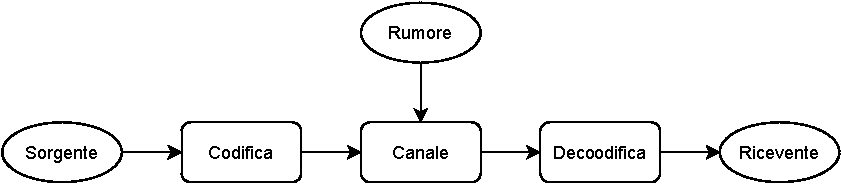
\includegraphics[width = \textwidth]{img/teo.pdf}
  \caption{Schema di un sistema generale di comunicazione tipico della teoria
    dell'informazione} 
  \label{fig:teo}
\end{figure}
Avendo:
\begin{itemize}
  \item la \textbf{sorgente} che produce segnali, dei simboli, che potrebbero
  essere continui (come la corrente), anche se noi li assumeremo come simboli di
  un alfabeto finito, avendo quindi una \textbf{sorgente discreta}
  \item i simboli, per poter essere spediti all'interno di un canale, vanno
  codificati, avendo una parte di \textbf{codifica}
  \item una volta codificati i simboli vanno nel \textbf{canale di
    trasmissione}, dove si ha del \textbf{rumore}. Tale \textit{rumore} prende
  un simbolo di quelli inseriti e lo cambia
  \item dal canale esce o il simbolo che è entrato o il simbolo modificato dal
  rumore e, tipicamente, non è immediatamente utilizzabile ma deve passare per
  una fase di \textbf{decodifica}
  \item il simbolo decodificato arriva al \textbf{destinatario}
\end{itemize}
Si hanno
alcune assunzioni sulla sorgente:
\begin{itemize}
  \item è \textbf{discreta}, i simboli emessi appartengono ad un alfabeto
  finito. Normalmente tali simboli sono $S=\{s_1, s_2,\ldots,s_q\}$
  \item i simboli vengono emessi uno alla volta ad ogni \textbf{colpo di
    clock}. Non si ha mai che in un colpo di clock non escano simboli o che ne
  escano più di uno solo 
  \item la sorgente è \textbf{senza memoria (\textit{memoryless})}, avendo che
  i simboli già usciti non influenzano per nulla il simbolo che sta per
  uscire. Ogni simbolo che esce non tiene conto del passato, \textit{è come se
    fosse il primo}
  \item è \textbf{probabilistica e randomizzata}. Si ha quindi che i simboli
  $S=\{s_1, s_2,\ldots,s_q\}$ escono con le probabilità
  $(p_1,p_2,\ldots,p_q)$. Deve valere che, ovviamente, che $p_i\in
  [0,1],\forall
  i=1,\ldots,q$. Si ha inoltre che le varie probabilità, nel loro insieme,
  devono formare una distribuzione di probabilità, avendo che:
  \[\sum_{i=1}^q p_i=1\]
  Potrei avere simboli con probabilità nulla di comparire ma nella pratica non
  è qualcosa di sensato. La sorgente la costruisco o da zero (e a quel punto
  un simbolo con probabilità nulla non lo metterei) o ho una sorgente che devo
  studiare (e qui potrei avere simboli con probabilità bassissime se non
  nulle, in tal caso bisognerebbe rivalutare l'assunzione dei simboli di
  quella sorgente). Possiamo quindi meglio dire che $p_i\in (0,1],\forall
  i=1,\ldots,q$.\\
  D'altro canto vedo se posso avere probabilità pari a 1 per un simbolo ma in
  tal caso avrei solo quello e non sarebbe interessante. Si ha quindi che:
  \[p_i\in (0,1),\forall i=1,\ldots,q\]
  \[\sum_{i=1}^q p_i=1\]
  \textit{Le sorgenti che emettono i simboli secondo  
    uno schema prefissato, deterministico, sono poco interessanti, avendo un
    comportamento banale}
\end{itemize}
Il concetto di \textit{spedire in un canale} può anche essere generalizzato in
altre ``idee'', come il disco su cui salvo dei dati e il tempo per cui li
salvo.\\ 
La parte di \textit{codifica e decodifica} può essere approfondita. Nello schema
in figura \ref{fig:teo} ci si è infatti concentrati sul canale, avendo che la
codifica serve a fare in modo che il simbolo trasmesso vada bene per essere
trasmesso nel canale. La \textbf{codifica} è a sua volta suddivisa in due parti:
\begin{enumerate}
  \item \textbf{codifica di sorgente}, che ha come obiettivo rappresentare nel
  modo più efficiente e compatto i simboli emessi dalla \textit{sorgente}. Si
  vuole quindi comprimere la sequenza di simboli (messaggi) emessi dalla
  sorgente, per impegnare meno banda possibile quando andremo a spedire. Si deve
  considerare che ogni bit in un file 
  compresso è essenziale per permettere di poter recuperare il contenuto
  compresso 
  \item \textbf{codifica di canale}, che ha quasi uno scopo opposto rispetto
  alla \textit{codifica di sorgente}, infatti ha come obiettivo quello di
  contrastare il rumore e per farlo aggiunge ridondanza al messaggio (da qui il
  discorso sull'obiettivo opposto)
\end{enumerate}
Si cerca quindi di comprimere il più possibile nella prima fase, quella di
\textit{codifica di sorgente} e di ridondare il meno possibile nella seconda,
quella di \textit{codifica di segnale}.\\
Per capire meglio quanto detto diamo alcune formalità.
\begin{definizione}
  Una \textbf{codifica} è una funzione $cod$ che prende i simboli della sorgente
  $S=\{s_1, s_2,\ldots,s_q\}$ e ad ogni simbolo $s_i$ gli assegna una stringa
  formata coi caratteri di un certo alfabeto $\Gamma$, l'\textbf{alfabeto
    della codifica}. Le stringhe di $\Gamma^*$ sono tutte quelle costruite
  sull'alfabeto $\Gamma$ di lunghezza arbitraria e finita, compresa la stringa
  vuota $\varepsilon$, che posso quindi formare coi simboli di $\Gamma$. Quindi
  ad ogni $s_i\in S$ assegno un $\gamma_i\in Gamma^*$, avendo che:
  \[cod:S\to \Gamma^*\]
  generalmente si ha che:
  \[|\Gamma|<|\Sigma|\]
  e quindi i simboli di $\Sigma$ sono mappati da $cod$ in  sequenze  di  simboli
  di $\Gamma$, a meno che non si ritenga accettabile il fatto che due o più
  simboli di $\Sigma$ vengano mappati nellostesso simbolo di $\Gamma$. \\
  \textit{Più avanti nel corso vedremo casi in cui $|\Gamma|>|\Sigma|$}
\end{definizione}
Si hanno quindi i simboli $S=\{s_1, s_2,\ldots,s_q\}$ che escono con
probabilità $(p_1,p_2,\ldots,p_q)$ e che vengono codificati con le stringhe
$\gamma_1,\gamma_2,\ldots,\gamma_q$. Le varie $gamma_i$ sono dette
\textbf{codeword}. Chiamando $l_i=|\gamma_i|$ la lunghezza 
di tali stringhe si ha che tali stringhe hanno associati i vari
$l_1,l_2,\ldots,l_q$.\\
L'obiettivo quindi della \textit{codifica di sorgente} è quello di minimizzare
la lunghezza media $L$ delle stringhe, avendo quindi una media pesata (pesata
sulle probabilità):
\[L=\sum_{i=1}^q p_i\cdot l_i\]
Tenendo conto delle probabilità, per minimizzare $L$, si deve, avendo a che fare
con termini che sono tutti $>0$ (avendo supposto che non si hanno probabilità
nulla e avendo che una codeword pari alla stringa vuota ha poco senso), fare in
modo che i termini siano tutti il più piccolo possibile. Dato che le probabilità
sono date mentre la codifica la sto costruendo, calcolando le codeword e di
conseguenza le loro lunghezze, devo fare in modo che se la probabilità è grande
la lunghezza deve essere piccola. Se invece la probabilità è piccola posso
permettermi una lunghezza più grande. Parto quindi dai simboli con probabilità
più grande e inizio a usare codeword più piccole possibili, usando via via
quelle più lunghe. \\
Un'idea simile è usata nel \textit{codice Morse} dove le
lettere meno comuni hanno le sequenze più lunghe di punti, linee e spazi (avendo
una codifica ternaria). La lettera più comune, la ``e'', ha infatti solo con un
punto, la codifica più breve mentre le meno comuni hanno sequenze multiple di
punti, linee e spazi che le separano (e gli spazi contano nella lunghezza di
queste codeword).\\
Noi non sappiamo in anticipo che messaggi verranno prodotti dalla sorgente e
quindi le codeword vanno studiate passo a passo, valutando i simboli più
probabili per associare le codeword più brevi e i meno probabili per le
codeword più lunghe.\\
Analizziamo meglio i codici, le codeword. Possono essere:
\begin{enumerate}
  \item \textit{a lunghezza fissa}, ovvero si ha che $l_1=l_2=\cdots=L_q$
  \item \textit{a lunghezza variabile}, avendo che ogni codeword può avere
  lunghezza diversa
\end{enumerate}
Ne segue quindi che il discorso di minimizzare $L$ ha senso solo in presenza di
\textit{codeword a lunghezza variabile} (potendo decidere per ogni simbolo che
codeword associare), avendo la \textbf{codifica a lunghezza variabile}.\\
Con \textit{codeword a lunghezza fissa} avrei tutte le $l_i$ uguali e quindi
avrei, avendo $l_i=l,\forall i$:
\[L=\sum_{i=1}^q p_i\cdot l_i \sum_{i=1}^q p_i\cdot l =l\cdot\sum_{i=1}^q
  p_i=l\cdot 1 = l\]
avendo, come facilmente intuibile, che la lunghezza media è la lunghezza fissa
stessa. Si hanno codifiche a lunghezza fissa, come banalmente numeri a 64bit
etc$\ldots$ in tal caso si parla di \textbf{codici a blocchi}.\\
Usando codifiche a lunghezza fissa si hanno anche esempi interessanti come
quello del \textit{codice pesato}, detto \textbf{codice pesato 01247}. Il nome
deriva dal fatto che si possono codificare le cifre da 0 a 9 (da 1 a 9 con poi
lo 0 dopo il 9) sotto forma di stringhe di 5 bit usando i pesi 0,1,2,4,7
associati a ciascun bit. Vediamo la tabella con la codifica di questo codice:
\begin{table}[H]
  \centering
  \begin{tabular}{c|ccccc} 
    & 0 & 1 & 2 & 4 & 7 \\
    \hline
    1 & 1 & 1 & 0 & 0 & 0 \\
    2 & 1 & 0 & 1 & 0 & 0 \\
    3 & 0 & 1 & 1 & 0 & 0 \\
    4 & 1 & 0 & 0 & 1 & 0 \\
    5 & 0 & 1 & 0 & 1 & 0 \\
    6 & 0 & 0 & 1 & 1 & 0 \\
    7 & 1 & 0 & 0 & 0 & 1 \\
    8 & 0 & 1 & 0 & 0 & 1 \\
    9 & 0 & 0 & 1 & 0 & 1 \\
    0 & 0 & 0 & 0 & 1 & 1
  \end{tabular}
\end{table}
Si nota che ogni codeword ha sempre 3 bit pari a 0 e due bit pari a 1, avendo un
\textbf{codice 2-su-5}. Banalmente i pesi si associano ai numeri 0,1,2,4,7 in
modo tale che essi, sommati, formino il numero voluto (ad esempio per 1 avrò i
pesi su 0 e 1, per 9 su 2 e 7 etc$\ldots$). L'unico caso è il caso dello 0, che
non può essere ottenuto come somma di due pesi (spesso si hanno nei codici casi
speciali da gestire a parte). Per lo 0 viene quindi presa una codeword non usata
per altri numeri e quindi l'unica scelta possibile è avere i pesi su 4 e 7
(visto che farebbe 11).\\
Su un totale ci 5 bit, avendo due bit a 1 e tre bit a 0, posso avere un numero
di codeword pari a:
\[n={{5}\choose{2}}=10\]
avendo che i 5 bit sono associati ai 5 elementi dove 1 segnala che ``sto usando
quel peso'', prendendo quindi i sottoinsiemi di due elementi a partire da un
insieme di cinque elementi, ovvero ``in quanti modi posso formare sottoinsiemi
che contengono due elementi a partire da un insieme di cinque elementi'' o detto
altrimenti ``quanti sono i modi in cui posso disporre due uni all'interno di una
stringa di cardinalità cinque''.\\
In un linguaggio di programmazione privo di una struttura dati dedicata posso
simulare un insieme di questo tipo tramite un vettore di bit (con 1 se
l'elemento associato all'indice c'è).\\
\textit{Il codice a barre è detto \textbf{codice 39} ed è un \textbf{codice
    3-su-9}}. \\
In merito alla \textbf{decodifica} si ha che anch'essa sarà di due tipi:
\begin{enumerate}
  \item \textbf{decodifica di canale}, vedendo e c'è stato un errore di
  trasmissione ed eventualmente correggendolo in automatico se il codice mi
  consente di farlo
  \item \textbf{ulteriore decodifica} che non è esattamente una \textit{codifica
    di sorgente} ma quanto una \textit{trasformazione}, dove le
  \textit{codeword} vengono trasformate nel formato leggibile dal
  \textbf{ricevente} 
\end{enumerate}
\section{Codici per individuare errori}
Ci concentriamo ora sulla \textit{codifica di canale} ignorando per ora la
\textit{codifica di sorgente}, avendo come obiettivo l'aggiunta di ridondanza a
simboli, che si suppongono già codificati con codeword, in modo tale che in
queste codeword, spedite nel canale dove eventualmente si possono avere
modifiche causate dal rumore, vengano eventualmente riconosciuti (ed
eventualmente corretti) errori in fase di \textit{decodifica}.\\
\textit{Parlando di codici per individuare errori solitamente, nei disorsi, si
  ha che $|\Gamma|<|\Sigma|$}
Qualora il ricevente con la sua decodifica si accorga che è successo qualcosa ma
non si è in grado di 
correggere quel qualcosa si hanno i cosiddetti \textbf{codici per individuare
  gli errori (\textit{error detection codes})}. Nel caso in cui il ricevente con
la sua decodifica si accorga dell'errore ci si chiede anche se può correggerlo
autonomamente senza chiedere che la sorgente spedisca nuovamente il
messaggio. Non sempre questa cosa si può fare ma quanto accade si parla di
\textbf{codici a correzione d'errore (\textit{error correction codes})}.
\subsection{Controllo di parità semplice}
Vediamo come capire se un messaggio ricevuto è valido.\\
Si supponga di spedire un pacchetto di $n$ bit (ma potrebbe essere qualsiasi
altra cosa ma per praticità prendiamo un bit) nel canale e che da esso esca un
certo pacchetto sempre di $n$ bit (per il rumore potrebbe non essere lo stesso).
\begin{definizione}
  Definiamo il \textbf{controllo di parità}. \\
  Avendo una sequenza di $n$ bits in
  cui si ha $n-1$ bits, dette \textbf{cifre di messaggio} di
  \textbf{messaggio vero}, che chiameremo
  \textbf{\textit{msg}} e un bit che è la \textbf{cifra di controllo}, che
  chiameremo \textbf{\textit{check}}. Le cifre di messaggio si indicano con
  $\circ$ mentre la cifra di controllo con $\times$ e quindi il messaggio è del
  tipo:
  \begin{table}[H]
    \centering
    \begin{tabular}{|c|c|c|c|c|c|c|}
      \hline
      $\circ$&$\circ$&$\circ$&$\circ$&$\cdots$&$\circ$&$\times$\\
      \hline
    \end{tabular}
  \end{table}
  avendo $n-1$ $\circ$ e un solo $\times$ (che potrebbe anche non essere in
  fondo, basta avere coscienza della posizione nel pacchetto, concordando la
  cosa tra mittente e ricevente).\\
  Si ha che:
  \begin{itemize}
    \item chi spedisce ha le cifre di messaggio e deve calcolare la cifra di
    controllo
    \item chi riceve controlla che la cifra di controllo sia coerente con le
    cifre di messaggio
  \end{itemize}
  Nell'\textbf{error detection code} il ricevente è solo in grado di capire che
  la sequenza non è valida ma per farlo bisogna assumere di avere limitazioni
  nella sequenza di $n$ bit che è entrata nel canale. Questa limitazione è che
  gli $n$ bit entranti nel canale siano una \textbf{codeword valida}, avendo
  che, preso un sottoinsieme $M$ di tutto l'insieme di $n$ bit, ovvero
  $M\subseteq\{0,1\}^n$, $M$ è un insieme di \textit{codeword valide}. Quindi
  solo un messaggio appartenente a $M$ può entrare nel canale. Fatta questa
  premessa, quando esce un messaggio, ho che, a causa del rumore, questo
  messaggio viene rovinato, non avendo più un messaggio
  valido (cosa che viene capita dal ricevente). \textit{Purtroppo può succedere
    che il rumore trasformi un messaggio valido in un altro messaggio valido ma
    non considereremo questa opzione per ora}. \\
  Nel \textbf{controllo di parità semplice} il pacchetto di $n$ bit, come visto
  è formato da $n-1$ bit di messaggio e un bit di controllo, la \textbf{check
    digit}. Si procede quindi, ricordando che siamo in un caso binario, a
  contare il numero di $1$ nei primi $n-1$ bit e se questo è dispari setto il
  bit di check a $1$ e si nota che così il numero di $1$ nel pacchetto intero
  di $n$ bit diventa pari, avendo la cosiddetta \textbf{parità pari} (ovvero
  ogni sequenza valida ha un numero pari di $1$). Controllando il numero di $1$
  il ricevente capisce se il rumore ha modificato il messaggio anche se non può
  capire cosa è successo (avendo quindi che il \emph{controllo di parità
    semplice} è solo un \emph{error detecting code} e non un \emph{error
    correcting code}). Non potendo fare nulla, in caso di errore identificato,
  il ricevente può solo chiedere al mittente di inviare nuovamente il messaggio.
  Qualora il rumore modificasse il messaggio in modo tale che si abbia comunque
  un numero apri di $1$ si rientrerebbe nella casistica sopra descritta in cui
  il rumore forma ancora un messaggio valido. Questa cosa può succedere se, nel
  caso binario, il rumore modifica un numero pari di cifre e quindi il
  \emph{controllo di parità semplice} funziona solo se viene modificato un
  \emph{numero dispari di cifre}.
  
\end{definizione}
Vediamo quindi meglio come calcolare la \textbf{check digit}.\\
Si rinominiamo gli $n$ bit come:
\[x_1x_2\cdots x_{n-1}\,y\]
quindi con $y$ \textit{check digit}.\\
Si ha che, con $\oplus$ \textit{xor}:
\[y=x_1\oplus x_2\oplus\cdots\oplus x_{n-1}\]
Ricordando che:
\begin{table}[H]
  \centering
  \begin{tabular}{c|c|c|c}
    $a$& $b$ & $a\land b$& $a\oplus b$\\
    \hline
    0 & 0 & 0 &0\\
    0 & 1 & 0 & 1\\
    1 & 0 & 0 &1\\
    1 & 1 & 1 & 0\\    
  \end{tabular}
\end{table}
quindi vale $1$ sse i due bit in input sono diversi ma questo non ci aiuta su
$n-1$ input. Altrimenti si ha che vale $1$ sse il numero di $1$ in input è
dispari e questo ci aiuta su $n-1$ input infatti la generalizzazione dello
\textit{xor} a più di due input è detta \textbf{funzione di parità}. Un altro
punto di vista per considerare lo \textit{xor} è quello della \textbf{somma a
  modulo 2} usando la notazione:
\[y=\bigoplus_{i=1}^{n-1}x_i=\sum_{i=1}^{n-1}x_i\bmod\,\, 2\]
avendo che faccio prima la somma e poi il modulo 2 mi dice 0 se è pari e 1 se è
dispari. \\
Si ha inoltre una relazione interessante tra le formule scritte usando solo
$\oplus$ e $\land$ nella cosiddetta \textbf{forma algebrica normale
  (\textit{ANF})}. Queste formule booleane possono essere trasformate in formule
aritmetiche con \textit{modulo 2}, quindi in $\mathbb{Z}_2$ dicendo che lo
\textit{xor} equivale alla \textit{formula modulo due} e l'\textit{and} al
\textit{prodotto modulo due} (la cosa vale in entrambi i versi).\\
La funzione di parità è così usata che in tutti i microprocessori, fin dagli
anni settanta, si ha un \textit{flag di parità} tra i flag della CPU, che viene
settato come appena visto a seconda dei bit caricati su un registro particolare
(a volte detto \textit{accumulatore}). Tale calcolo è facilmente mappabile in
un circuito, avendo che lo \textit{xor} gode della proprietà associativa (avendo
un circuito che fa un albero di porte \textit{xor}).

Posso anche simulare lo \textit{xor} con un \textbf{automa a stati finiti}, con
due stati ``pari'' e ``dispari'', con il ``pari'' stato iniziale (diciamo che
input vuoto è pari):
\begin{center}
  \begin{tikzpicture}[shorten >=1pt,node distance=3cm,on grid,auto]
    \node[state, initial, accepting] (q_0) {$pari$};
    \node[state, accepting] (q_1) [right=of q_0] {$dispari$};
    \path[->]
    (q_0) edge [bend left = 25] node {1} (q_1)
    edge [loop above] node {0} ()
    (q_1) edge [bend left = 25] node {1} (q_0)
    edge [loop right] node {0} ();
  \end{tikzpicture}
\end{center}
Questo metodo ha senso se il canale è pochissimo rumoroso, avendo pochissima
probabilità di avere la modifica di un bit e ancora meno di due (due modifiche
si ricorda che non verrebbero rilevate essendo pari), così poca da poter
ipotizzare che non avvengano mai due errori (e se mai dovesse succedere
bisognerà valutare l'impatto del problema e le conseguenze). Stiamo assumendo
quindi che la \textbf{probabilità d'errore} può essere \textbf{trascurabile}
infatti canali di buona qualità dovrebbero sbagliare non più di un bit su un
milione, per canali più affidabili anche uno su un miliardo. Possiamo quindi
trascurare che possano accadere due errori e dire che il \textbf{controllo di
  parità} va bene. \\
Parliamo ora meglio di \textbf{ridondanza}, definendola formalmente.
\begin{definizione}
  La \textbf{ridondanza} $R$ è definita come:
  \[R=\frac{\mbox{il numero totale di simboli/cifre spediti}}{\mbox{numero di
        simboli/cifre che sono effettivamente parte del messaggio}}\] 
  Nel caso del \emph{controllo di parità} i simboli che vogliamo spedire sono
  $n$ bit a fronte di $n-1$ bit di vero messaggio. Si ha quindi:
  \[R=\frac{n}{n-1}=\frac{(n-1)+1}{n-1}=1+\frac{1}{n-1}\]
  Mettendo in evidenza che la ridondanza è sempre $R\geq 1$, visto che a
  numeratore abbiamo almeno una cifra in più (quella della \emph{check digit}) e
  che quindi è sicuramente maggiore del denominatore. In realtà per avere $R=1$
  dovrei avere numeratore e denominatore uguali che non ha molto senso parlando
  di ridondanza, quindi nei casi \emph{interessanti} si ha che $R>1$. Guardando
  la formula la cosa è confermata da $1+\frac{1}{n-1}$ con $\frac{1}{n-1}$ che
  viene detto \textbf{eccesso di ridondanza}.
\end{definizione}
\begin{definizione}
  Possiamo \textbf{generalizzare} la definizione di \textbf{ridondanza},
  indicando $tot=msg+check$:
  \[R=\frac{msg+check}{msg}=\frac{tot}{msg}\]
  avendo:
  \begin{itemize}
    \item $msg$ numero di simboli/cifre di messaggio
    \item $check$ numero di cifre di controllo
  \end{itemize}
  Ma allora (avendo $check<msg$ per avere qualcosa di sensato):
  \[R=\frac{msg+check}{msg}=1+\frac{check}{msg}\]
  che è la forma ``generale'' della ridondanza. Si ha che $\frac{check}{msg}$ è
  \textbf{eccesso di ridondanza}. 
\end{definizione}
\textit{Si può dire di non avere necessità di ``proteggere'' di più il bit di
  parità in quanto, per la macchina, conta come tutti gli altri. Tutti vanno
  ``protetti'' nello stesso modo.}\\
\textit{Come ho la \textbf{parità pari} potrei avere la \textbf{parità dispari},
dove i messaggi validi hanno un numero dispari di $1$. I vari ragionamenti sono
analoghi, essendo tutto uguale dal punto di vista matematico, avendo un
isomorfismo tra le due tecniche. La scelta tra i due dipende dai casi è dalla
celta di cosa rappresentiamo con $0$ e $1$ (pensiamo con $0$ che rappresenta
assenza di segnale, in questo caso meglio usare la parità dispari, mentre se $0$
e $1$ rappresentassero diverse quantità di Volt andrebbe bene la parità
pari)}. \\ 
\textbf{Nel corso si userà comunque solo la \textit{parità pari}}.
\subsection{Il rumore bianco}
Introduciamo ora un primo \textit{modello di rumore}, il \textbf{modello del
  rumore bianco}.
\begin{definizione}
  Un \textbf{modello di rumore} è un modello matematica che descrive cosa
  succede nel canale quando il rumore rovina i bit.
\end{definizione}
\begin{definizione}
  Il \textbf{modello del rumore bianco} consiste nell'avere il messaggio con i
  bit $x_1x_2\cdots x_n$ (con magari $x_n$ come controllo di parità ma dato che
  ``i bit non sono colorati'' la cosa non ci interessa davvero) e avere una
  certa probabilità $p$. Si hanno due condizioni:
  \begin{enumerate}
    \item si ha che $p\in(0,1)$ che è la probabilità che avvenga
    un errore in ogni posizione $i\in [1,n]$ del messaggio. Si ha quindi che la
    probabilità $p$ è uguale in tutte le posizioni
    \item le posizioni sono tutte indipendenti, ovvero il fatto che magari si ha
    un errore nella posizione $i$ non influisce sulle altre. Avendo quindi
    l'eventi casuale $E_i$ con:
    \[E_i=\mbox{è avvenuto un errore in i}\]
    allora:
    \[E_i\mbox{ ed }E_j \mbox{ sono indipendenti, }\forall i\neq j\]
  \end{enumerate}
  \textbf{Le due proprietà sopra elencate rendono molto semplice il modello}.\\
  Questo però non è molto realistico, basti pensare al rumore dovuto ad uno
  sbalzo di corrente, dove da un bit in poi e per diversi bit si avranno alte
  probabilità d'errore. Quando l'errore influisce su una certa porzione di bit
  si dice che si ha un \textbf{burst di errori} (che non può essere gestito con
  le tecniche per il \textit{rumore bianco}, anche se si riesce con qualche
  workaround).\\
  Si è visto che $p\in(0,1)$ infatti:
  \begin{itemize}
    \item se si avesse $p=0$ si avrebbe che ogni bit arriverebbe sempre
    corretto, ma questo può avvenire solo in un mondo utopico e non in quello
    reale/fisico. Non esiste un canale reale non affetto da errori, quindi si ha
    $p\neq 0$
    \item se si avesse $p=1$ si avrebbe che ogni bit del messaggio arriverebbe
    errato ma questa non sarebbe una brutta situazione, anzi sarebbe ottima
    infatti mi basterebbe avere una porta logica \textit{not} della linea di
    trasmissione per riottenere il messaggio corretto, ottenendo un canale $p=0$
    d'errore. Anche questo però è irrealistico quindi $p\neq 1$ 
  \end{itemize}
  Supponiamo ora che $p>\frac{1}{2}$ quindi ho più probabilità che un bit arrivi
  sbagliato che giusto. Anche in questo caso una porta logica \textit{not} alla
  fine della linea di trasmissione per ottenere un canale con $1-p$ come
  probabilità d'errore. Quindi anche questo non ha molto senso quindi si
  considera che:
  \[p\in(0,\frac{1}{2})\]
  Manca solo da valutare $p=\frac{1}{2}$. \\
  Con $p=\frac{1}{2}$ si ha che il bit
  di output è completamente causale e indipendente da cosa sia stato spedito. È
  come se il canale generasse $n$ bit casuali con probabilità uniforme
  ($\frac{1}{2}$), avendo un cosiddetto \textbf{canale completamente
    rumoroso}. Dal punto di vista pratico sarebbe interessante un tale canale,
  per altri punti di vista (come quello della crittografia), avendo infatti un
  \textbf{generatore di bit completamente casuali}. Purtroppo questo non si può
  fare quindi si assume $p\neq \frac{1}{2}$.
\end{definizione}
Cerchiano di capire quale sia la probabilità che avvengano $k$ errori con $0\leq
k\leq n$ (quindi da nessun errore a tutti gli $n$ bit errati), che indichiamo
con: 
\[p[\mbox{ k errori }]\]
Valutiamo i vari casi:
\begin{itemize}
  \item partiamo con 1 errore, quindi $k=1$, avendo $p[\mbox{ 1 errori }]$.\\
  Questo significa che per il messaggio di $n$ bit si immagina un vettore di bit
  associato con $0$ e $1$ come
  ``bandierine'' che indicano se è avvenuto un errore o no in una certa
  posizione. Quindi se in un 
  certa posizione ho $0$ diciamo che significa che non ho un errore di
  trasmissione mentre se ho $1$ ho un errore. Il messaggio di $n$ bit diventa
  quindi una sorta di \textit{maschera} che con gli $1$ mi dice dove è avvenuto
  l'errore. Se suppongo che ne è avvenuto uno solo avrò un solo $1$ e bisogna
  calcolare la  probabilità che questo avvenga.\\
  Supponga che l'errore sia al primissimo bit, quindi in posizione $i=1$, avendo
  quindi, per il discorso delle ``bandierine'' che $msg=10000\ldots 0$ e quindi
  si ha, avendo che la probabilità che avvenga la trasmissione avvenga
  correttamente è $1-p$ (cosa che avviene $n-1$ volte), mentre $p$ che avvenga
  sbagliata (cosa che avviene una sola volta):
  \[p[\mbox{ 1 errori }]=p^1\cdot(1-p)^{n-1}=p\cdot(1-p)^{n-1}\]
  \textbf{Posso fare $\cdot$ in quanto si è supposta l'\textit{indipendenza}
    (non avendo intersezioni tra gli eventi)}.\\
  Ma questo non sta considerando tutto ma solo la prima posizione. Completando
  il calcolo avendo di volta in volta in somma la probabilità di un errore nella
  posizione $i$ ho che:
  \[p[\mbox{ 1 errori }]=p^1\cdot(1-p)^{n-1}+(1-p)^1\cdot
    p^1\cdot(1-p)^{n-2}+\cdots\]
  ma questo conto si può semplificare, avendo sempre gli stessi termini che si
  ripetono:
  \[p[\mbox{ 1 errori }]=n\cdot p^1\cdot(1-p)^{n-1}=n\cdot p\cdot(1-p)^{n-1}\]
  Infatti so che $p\cdot(1-p)^{n-1}$ è la probabilità di avere un errore in una
  certa 
  posizione fissata. Mi chiedo dove posso mettere questa posizione in tutti i
  modi possibili nel pacchetto di $n$ bit e ho che, avendo un solo errore, ho
  $n$ modi per posizionarlo, ciascuno con probabilità $p\cdot(1-p)^{n-1}$
  
  \item passiamo a due errori, avendo $p[\mbox{ 2 errori }]$.\\
  Ho un ragionamento analogo. Parto supponendo di avere i due errori nelle prime
  due posizioni del messaggio/pacchetto, avendo quindi 1 nelle prime due
  posizioni della maschera. Abbiamo comunque già visto che poi il ragionamento
  si generalizza per qualsiasi posizione, in questo caso coppie (anche non
  consecutive) di posizioni. Si ha che, ipotizzando che le prime due siano
  errate:
  \[p[\mbox{ 2 errori }]=p^1\cdot p^1\cdot(1-p)^{n-2}=p^2\cdot(1-p)^{n-2}\]
  Ma anche qui dobbiamo vedere la probabilità per qualsiasi coppia, facendo
  variare le due posizioni d'errore in tutti i modi possibili ma questo è come
  prendere un qualsiasi sottoinsieme di due elementi a partire da un insieme di
  $n$ elementi ma questo altro non è che il calcolo che si fa tramite il
  coefficiente binomiale, avendo quindi:
  \[p[\mbox{ 2 errori }]={{n}\choose{2}}\cdot p^2\cdot(1-p)^{n-2}\]
  \item analogamente a quanto fatto per due errori potrei fare con tre,
  quattro, etc$\ldots$
  \item possiamo generalizzare con $k$ errori, avendo $p[\mbox{
    k errori }]$.\\
  Si hanno quindi $k$ uni da disporre in tutti i modi possibili nel vettore di
  $n$ bit. Si ha quindi:
  \[p[\mbox{ k errori }]={{n}\choose{k}}\cdot p^k\cdot(1-p)^{n-k}\]
  E quindi posso valutare la cosa nei due casi estremi:
  \begin{itemize}
    \item $k=0$, avendo 0 errori. Ho un solo modo per mettere zero $1$ nella
    maschera di bit (da nessuna parte) e infatti (avendo poi tutti gli $n$ bit
    la stessa probabilità di uscire corretti): 
    \[p[\mbox{ 0 errori }]={{n}\choose{0}}\cdot p^0\cdot(1-p)^{n-0}=1\cdot
      1\cdot (1-p)^n=(1-p)^n\]
    \item $k=n$, avendo $n$ errori\footnote{Su dispense del prof grafico con
      $n=8$, $p=0.1$ e $k$ che varia tra 0 e 8}. Ho un solo modo per mettere
    tutti $1$ nella  maschera di bit (ovunque) e infatti (avendo poi tutti gli
    $n$ bit la stessa probabilità di uscire errati):
    \[p[\mbox{ n errori }]={{n}\choose{n}}\cdot p^n\cdot(1-p)^{n-n}=1\cdot
      p^n\cdot 1=p^n\]
  \end{itemize}
  \textit{Si nota che i due casi estremi sono ``speculari''}.
\end{itemize}
\textit{In questo elenco puntato si è quindi ragionato sulle celle della
  maschera di bit associata al pacchetto e non del pacchetto in se, anche se
  spesso risulti ambiguo}.\\
Consideriamo ora nuovamente $p[\mbox{ 1 errore }]$, si ha che, dalla
generalizzazione è:
\[p[\mbox{ 1 errore }]={{n}\choose{1}}\cdot p^1\cdot(1-p)^{n-1}=n\cdot p\cdot
  (1-p)^{n-1}\]
Introduciamo un'approssimazione interessante dell'analisi matematica che vale
per $\alpha\in \mathbb{R}$ e $|X|<1$, ovvero $-1<x<1$:
\[(1+x)^\alpha\simeq 1+\alpha\cdot x\]
Ovvero $1+\alpha\cdot x$ sono i primi due termini dello sviluppo in serie di
$(1+x)^\alpha$.\\
Tratto quindi la formula per un errore in base a questa approssimazione:
\[p[\mbox{ 1 errore }=n\cdot p\cdot(1-p)^{n-1}\simeq n\cdot p\cdot
  [1-p\cdot(n-1)]=n\cdot p-n^2\cdot p^2+n\cdot p^2\]
Ma so che $p\in(0,1)$ e quindi $p^2<p$, infatti (\textit{grafico
  approssimativo}): 
\begin{figure}[H]
  \centering
  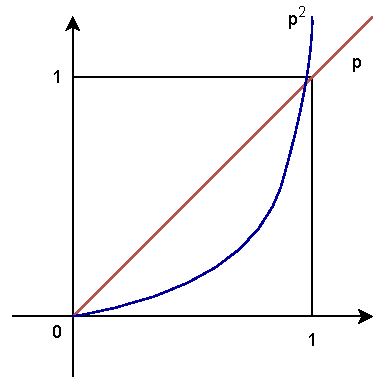
\includegraphics[scale = 0.8]{img/p.pdf}
\end{figure}
ma quindi, sempre approssimando (avendo quindi già due approssimazioni):
\[p[\mbox{ 1 errore }=n\cdot p\cdot(1-p)^{n-1}\simeq n\cdot p-n^2\cdot
  p^2+n\cdot p^2\simeq n\cdot p\]
Quindi:
\[p[\mbox{ 1 errore }\simeq n\cdot p\]
Analogamente ragiono per due errori:
\[p[\mbox{ 2 errori }]={{n}\choose{2}}\cdot
  p^2\cdot(1-p)^{n-2}\simeq{{n}\choose{2}}\cdot
  p^2\cdot[1-p\cdot(n-2)]={{n}\choose{2}}\cdot (p^2-n\cdot p^3+2p^3)\]
Ma anche qui si ha che $p\in(0,1)$ e quindi $p^3<p$, e quindi si ha:
\[p[\mbox{ 2 errori }]\simeq{{n}\choose{2}}\cdot p^2=\frac{n\cdot
    (n-1)}{2}\cdot p^2\]
In generale, per $k$ errori, con gli stessi passaggi:
\[p[\mbox{ k errori }]\simeq{{n}\choose{k}}\cdot p^k\]
\textbf{I conti diventano molto più semplici}.\\
Si è detto che se la probabilità di due errori è piccoli si può decidere di
trascurarla (usando poi solo il \textit{controllo di parità semplice}). Da
queste approssimazioni vediamo che la probabilità di un errori è $\simeq n\cdot
p$ mentre per due $\simeq\frac{n\cdot (n-1)}{2}\cdot p^2$. Se ipotizziamo $p\sim
10^{-6}$, quindi uno su un milione, si ha che $p^2=10^{-12}$ quindi assolutamente
trascurabile. Si segnala comunque che questa non è una pratica standard.
Normalmente si hanno, ad esempio, \textbf{low density parity codes (LDPC)} dove
si sparano a caso vari controlli di qualità nell'ottica di mantenere le
proprietà di correzione degli errori usando meno controlli possibile, avendo,
tornando alla ridondanza $R=1+\frac{check}{msg}$, che si vuole usare il minor
numero di cifre di controllo per abbassare l'\textit{eccesso di ridondanza},
abbassando la ridondanza stessa, avvicinandosi quindi a $1^+$ (ci si avvicina
da destra ovviamente). Riducendo l'\textit{eccesso di ridondanza} si ha che
ogni cifra di controllo \textit{copre/protegge} il maggior numero ci
simboli/cifre del messaggio. \textit{A parità di simboli inviati si vuole quindi
  ridurre il numero di cifre di controllo}.\\
Approfondiamo e usiamo quindi il\textit{ modello del rumore bianco} per vedere
qual è a probabilità che il ricevente non riesca a capire che c'è stato un
errore utilizzando il \textit{controllo di parità semplice}.\\
Ricordiamo che il messaggio è della forma:
\[x_1x_2\cdots x_{n-1}y\]
con $y$ \textit{controllo di parità semplice} calcolato come:
\[y=\bigoplus_{i=1}^{n-1}x_i\]
Un numero dispari di errore mi segnala che ci sono stati problemi, usando la
\textit{parità pari} (i pacchetti inseriti nel canale hanno un numero apri di
$1$).\\ 
Vogliamo quindi la probabilità che il controllo di parità fallisca, ovvero:
\[p[\mbox{ controllo }\bigoplus \mbox{ fallisce }]\]
ma questo è uguale alla probabilità che avvenga un numero pari di errori
(\textbf{zero escluso}, ovviamente):
{\footnotesize{\[p[\mbox{ controllo }\bigoplus \mbox{ fallisce }]=p[\mbox{ numero
      pari di errori }]=p[\mbox{ 2 errori }]+p[\mbox{ 4 errori }]+\cdots \]}}
Diciamo che, per comodità:
\[1=(1-p)+p=[(1-p)+p]^n\]
Ma so che $(a+b)^n=\sum_{k=0}^n{{n}\choose{k}}a^{n-k}b^k$, quindi:
\[1=[(1-p)+p]^n=\sum_{k=0}^n{{n}\choose{k}}(1-p)^{n-k}p^k\]
ma questa è ${{n}\choose{k}}(1-p)^{n-k}p^k=p[\mbox{ k errori }]$ (infatti la
somma di tutte le probabilità è appunto 1), quindi:
\[1=[(1-p)+p]^n=\sum_{k=0}^n{{n}\choose{k}}(1-p)^{n-k}p^k=\sum_{k=0}^np[\mbox{
    k errori }]\]
D'altro canto posso anche dire che, sempre applicando l'espansione di $(a+b)^n$,
scomponendo però $(-p)^k$ in $(-1)^k\cdot p^k$ (dove $(-1)^k$ vale $1$ per k
pari e $-1$ per $k$ dispari). Si ha quindi:
\[(1-2\cdot p)^n=[(1-p)-p]^n=\sum_{k=0}^n(-1)^k\cdot {{n}\choose{k}}\cdot
  p^k\cdot(1-p)^{n-k}\]
Ma quindi ho:
\[(1-2\cdot p)^n=
  \begin{cases}
    {{n}\choose{k}}\cdot  p^k\cdot(1-p)^{n-k} &\mbox{sse $k$ è pari}\\
    -{{n}\choose{k}}\cdot  p^k\cdot(1-p)^{n-k} &\mbox{sse $k$ è dispari}\\
  \end{cases}
\]
Quindi se $k$ è dispari le espansioni di $1$ e $(1-2\cdot p)^n$ sono uguali ma
di segno opposto mentre se $k$ è pari sono uguali con lo stesso segno. Ma quindi
questa somma delle due espansioni mi lascia col doppio dei soli termini con $k$
pari che ci aiuta volendo calcolare proprio le probabilità con un numero di
errori pari. Si ha quindi, dividendo già per due avendo il discorso del doppio:
\[\frac{1+(1-2\cdot p)^n}{2}=\sum_{t=0}^{\lfloor \frac{n}{2}\rfloor}
  {{n}\choose{2\cdot t}}\cdot p^{2t}\cdot(1-p)^{n-2t}\]
La somma va quindi da 0 alla parte intera di $\frac{n}{2}$. Nel coefficiente
binomiale ho $2\cdot r$ che è una quantità sicuramente pari. In generale è come
se avessi $k=2\cdot t$ ciclando solo sui $k$ pari. Ho quindi ottenuto:
\[p[\mbox{ 0 errori }]+p[\mbox{ 2 errori }]+p[\mbox{ 4 errori }]+\cdots \]
Non vogliamo però $t=0$ quindi:
{\footnotesize{\[p[\mbox{ controllo }\bigoplus \mbox{ fallisce }]=p[\mbox{
        numero pari di errori }]=\frac{1+(1-2\cdot 
    p)^n}{2}-p[\mbox{ 0 errori }]\]}}
\[=\frac{1+(1-2\cdot p)^n}{2}-  {{n}\choose{0}}\cdot
  p^{0}\cdot(1-p)^{n-0}=\frac{1+(1-2\cdot p)^n}{2}-(1-p)^n\]
E quindi:
{\small{\[p[\mbox{ controllo }\bigoplus \mbox{ fallisce }]=p[\mbox{ numero pari
        di errori }]=\frac{1+(1-2\cdot p)^n}{2}-(1-p)^n\]}}
D'altro canto potrei anche calcolare $p[\mbox{ numero dispari di errori }]$:
\[p[\mbox{ numero dispari di errori }]=1-p[\mbox{ numero pari di errori }]\]
(\textit{o anche modificando la sommatoria per ciclare sui $k$ dispari}).\\
Facendo qualche conto\footnote{i calcoli
  per il numero dispari di errore sono materiale extra sulle dispense del
  docente} si ottiene che: 
\[p[\mbox{ numero dispari di errori }]=1-(p[\mbox{ numero pari di errori
  }]+p[\mbox{ 0 errori }])\]
ovvero:
\[p[\mbox{ numero dispari di errori }]=\frac{1-(1-2\cdot p)^n}{2}\]
\textit{In generale il numero dispari di errori è meno interessante}.\\
\subsection{Gestione dei burst}
Come abbiamo introdotto con il solo \textit{controllo di parità} e con
il \textit{rumore bianco} non si possono gestire i \textbf{burst di
  errori}. Vediamo quindi un modo semplice per gestirli.\\
Si supponga di voler spedire dei messaggi formati da lettere, ad esempio:
\begin{table}[H]
  \centering
  \begin{tabular}{|c|c|c|c|}
    \hline
    c&i&a&o\\
    \hline
  \end{tabular}
\end{table}
Posiamo di rappresentare ogni lettera tramite l'\textbf{ASCII standard} a 7 bit:
\begin{table}[H]
  \centering
  \begin{tabular}{c|c}
    char & bit\\
    \hline
    c&1000011\\
    i&1001001\\
    a&1000001\\
    o&1001111
  \end{tabular}
\end{table}
Si supponga di avere dei burst di errori di lunghezza $L$ e per semplicità
assumo $L$ di lunghezza pari alle singole word, quindi $L=7$. Per gestire il
burst spedisco prima i 7 bit della prima lettera poi quelli della seconda
etc$\ldots$\\
Infine spedisco un intero pacchetto di bit di controllo di 7 bit dove ogni bit
viene calcolato controllando quella posizione di bit in tutti i pacchetti
precedenti, sempre tramite lo \textit{xor}. Nel caso d'esempio si ha quindi, con
$x$ per indicare il \textbf{check} (se nella colonna sopra ho un numero apri di
$1$ metto $0$ altrimenti $1$):
\begin{table}[H]
  \centering
  \begin{tabular}{c|c}
    c&1000011\\
    i&1001001\\
    a&1000001\\
    o&1001111\\
    \hline
    x&0000100\\
  \end{tabular}
\end{table}
Suppongo un burst che rovini dalla posizione 2 alla 4 incluse (avendo che quindi
molto probabilmente non ci torneranno i conti facendo il check su
$x[2,4]=000$).\\
Ovviamente anche qui un numero pari di errori inganna il sistema avendo comunque
un \textit{controllo di parità semplice} e anche in caso d'errore il ricevente
non sa comunque dove sia avvenuto e quindi fa \textbf{detection} ma non può fare
\textbf{correction}.
\subsection{Codici pesati}
Abbiamo già parlato del \textbf{codice 01247} vediamo ora un codice pesato più
interessante e utilizzato.\\
\begin{definizione}
  Definiamo questo \textbf{codice pesato} come un codice per cui si hanno alcune cifre
  di messaggio $msg=m_1m_2\cdots m_nc$ alle quali associamo dei pesi che
  dipendono dalla posizione in cui si trovano le varie cifre. In particolare si
  ha peso:
  \begin{itemize}
    \item $1$ per la \textbf{check digit} $c$
    \item $2$ per $m_n$
    \item si prosegue sempre aumentando di 1 per le altre cifre
    \item $n$ per $m_2$
    \item $n+1$ per $m_1$
  \end{itemize}
\end{definizione}
Questo si fa perché la cifra di controllo è calcolata per far ottenere:
\[m_1\cdot (n+1)+m_2\cdot n+\cdots+m_n\cdot 1+c\cdot 1=0\]
ma ovviamente questo non sembra possibile e infatti i conti sono fatti in
\textbf{modulo numero primo}, avendo per esempio, se scegliamo come numero
prima $37$:
\[m_1\cdot (n+1)+m_2\cdot n+\cdots+m_n\cdot 1+c\cdot 1\equiv 0\bmod\,\, 37\]
La scelta di 37 non è causale, infatti volendo:
\begin{itemize}
  \item rappresentare le 21 lettere dell'alfabeto inglese
  \item rappresentare dieci cifre da 0 a 9
  \item un simbolo per lo spazio
\end{itemize}
e quindi siamo a 32 simboli e ci serve un numero primo $\geq 31$ e quindi va
bene 37.\\
Vogliamo un numero prima perché se vogliamo fare i conti con le congruenze è
più semplice farle in \emph{modulo numero primo}.\\
Lavoriamo quindi nella classe dei resti:
\[[0]_{37},[1]_{37},\ldots, [36]_{37}\]
e in questo modo se facciamo le varie operazioni è tutto uguale al solito fino
a 36 (cosa che non succede per le classi dei resti in modulo non numero
primo).\\
La classe dei resti in modulo numero primo è un \textbf{campo} mentre se non
fosse primo si avrebbe un \textbf{anello}. In un campo se $x\cdot y=0$ o che
$x=0$ oppure $y=0$ (cosa che non succede negli anelli). Inoltre in un campo ho
che se $x\cdot y =z$ allora $x=z\cdot y^{-1}$ (in un anello non per tutti gli
$y$ esiste un $y^{-1}$ mentre in un campo sì).\\
Facendo dipendere il calcolo del peso della \textbf{check digit} da tutti gli
altri pesi perché, così facendo, sopratutto nelle comunicazioni di tipo
\textbf{seriale} (dove si spedisce una cifra alla volta), ci si accorge subito
se una cifra è andata persa oppure se si è aggiunta cifra o se due cifre si
sono scambiate (cosa comunque difficile in un sistema di comunicazione
elettronico ma è utile in altre situazioni, sopratutto di conti ``a
mano'').\\
Si supponga di avere delle cifre $b$ e $a$, la prima con peso $k+1$ e la
seconda con peso $k$, avendo una scrittura del tipo $cifra(peso)$:
\[b(k+1)+a(k)\]
Ipotizziamo di scambiare $a$ e $b$ (ora $a$ pesa $k+1$ e $b$ pesa $k$),
avendo:
\[a(k+1)+b(k)\]
Ma facendo la differenza si nota che non è nulla:
\[[b(k+1)+a(k)]-[a(k+1)+b(k)]\neq 0\]
infatti ho:
\[b\cdot k+b+a\cdot k-a\cdot k-a-b\cdot k=b-a\]
ma $b-a=0$ sse $b=a$ e quindi l'unico caso in cui non ci si accorge dello
scambio è avere lo scambio di due cifre uguali che non fa cambiare il
risultato.\\
Questa idea viene usata anche nei codici a barre. Vediamo quindi un algoritmo
per calcolare la cifra di controllo:
\begin{algorithm}[H]
  \begin{algorithmic}
    \Function{CheckCalc}{}
    \State $sum \gets 0$
    \State $ssum \gets 0$
    \While {\textit{not} EOF}
    \State \textbf{read} \textit{sym}
    \State $sum \gets sum+sym\,\,\, (\bmod\,\, 37)$
    \State $ssum \gets ssum+sum\,\,\, (\bmod\,\, 37)$
    \EndWhile
    \State $temp \gets ssum+sum\,\,\, (\bmod\,\, 37)$
    \State $c \gets 37-temp\,\,\, (\bmod\,\, 37)$
    \State \textbf{return} $c$ 
    \EndFunction
  \end{algorithmic}
  \caption{Algoritmo di calcolo dei pesi per codice pesato}
\end{algorithm}
Dove:
\begin{itemize}
  \item $sum$ tiene conto della somma numerica della nostro calcolo, accumulando
  i vari termini 
  \item $ssum$ che è una \textit{somma delle somme} e tiene conto implicitamente
  dei vari persi che crescono spostandoci da destra a sinistra come visto
  sopra. Si accumulano i termini e i loro pesi
\end{itemize}
\textit{I $\bmod 37$ nel ciclo sono in realtà superflui ma conviene farli per
  non far diventare i numeri troppo grossi. Le ultime due operazioni servono a
  risolvere alcune problematiche che non vediamo qui.}\\
Vediamo una più chiara simulazione.
\begin{esempio}
  Avendo, simulando per un messaggio $wxyzc$, con $c$ \textit{check digit}:
  \begin{table}[H]
    \centering
    \begin{tabular}{|c|c|c|}
      \hline
      msg & sum & ssum \\
      \hline
      $w$ & $w$ & $w$ \\
      $x$ & $w+x$ & $2\cdot w+x$ \\
      $y$ & $w+x+y$ & $3\cdot w+2\cdot x+y$ \\
      $z$ & $w+x+y+z$ & $4\cdot w+ 3\cdot x+2\cdot y+z$ \\
      \hline
      $c$ & $w+x+y+z+c$ & $5\cdot w+4\cdot x+3\cdot y+2\cdot z+c$ \\
      \hline
    \end{tabular}
  \end{table}
  Arrivato alla fine voglio calcolare $c$ in modo che:
  \[5\cdot w+4\cdot x+3\cdot y+2\cdot z+c \equiv 0 \bmod\,\, 37\]
\end{esempio}
Il mittente ha un messaggio e ci calcola la \textbf{check digit}.
Chi riceve fa lo stesso calcolo e alla fine controlla la \textbf{check
  digit}. Un altro modo per il ricevente è quello di fare solo l'ultimo calcolo
se farli tutti step by step.\\
Introduciamo un particolare tipo di codice, quello \textbf{ISBN
  (\textit{(International Standard BookNumber})} dei libri, che 
sono legati, per il codice a barre, allo standard europeo \textbf{EAN13} (negli
USA si usa lo standard 
\textbf{UPC}). In questo codice si hanno 10 cifre (con al più il carattere $X$)
che un identificano in modo univoco ad un libro. Nel dettaglio:
\begin{itemize}
  \item la prima cifra rappresenta lo stato in cui è stampato il libro. Questo
  ha problemi non avendo solo 9 stati che producono libri
  \item le successive 2 cifre sono le prime due per l'editore, anche questo è un
  problema in quanto alcuni stati hanno più di 100 case editrice
  \item le successive 6 sono il numero del libro
  \item l'ultima cifra è il checksum, la check digit
\end{itemize}
In realtà ho trattini dopo la prima cifra, dopo la quinta e dopo la nona ma non
contano nulla ai fini del calcolo ma sono aiutati solo per facilitare la
leggibilità dello stesso.\\
\textbf{A causa dei problemi sopra descritti i codici ISBN vengono assegnati
  ormai con libertà dalle case editrici, usando il primo codice libero}.\\
ISBN è un codice pesato dove i conti sono
fatti in $\bmod\,\,\,11$ (il più piccolo numero primo più grande di 10). Potrei
avere come risultato 10 avendo $\bmod\,\,\,11$ ma in quel caso uso $X$ come
checksum, come ultima cifra.
\begin{esempio}
  Prendiamo l'ISBN:
  \[0\mbox{-}1315\mbox{-}2447\mbox{-} x\]
  e vogliamo verificare che sia effettivamente $X$. Si ha (con $\equiv$ indico i
  conti $\bmod\,\,\,11$):
  \begin{table}[H]
    \centering
    \begin{tabular}{|c|c|c|}
      \hline
      msg & sum & ssum \\
      \hline
      0 & 0 & 0\\
      1 & 1 & 1\\
      3  & 4 & 5\\
      5 & 10 & $20\equiv 9$\\
      2& $12\equiv 1$ & $21\equiv 10$\\
      4 & 5 & $15\equiv 4$\\
      4 & 9 & $13\equiv 2$\\
      7 & $16\equiv 5$ & 7\\
      \hline
      $X\equiv 10$ & $15\equiv 4$ & $11\equiv 0$\\
      \hline
    \end{tabular}
  \end{table}
  Avendo che effettivamente la somma $\bmod\,\,\,11$ fa 0 e quindi è
  verificato.\\ 
  Avrei inoltre, per l'algoritmo, controllando la check digit:
  \[temp = 7+5=12\equiv 1\]
  \[c=11-1=10\equiv X\]
\end{esempio}
\section{Codici per correggere errori}
In questo caso il ricevente non solo deve capire dove è l'errore ma deve anche
correggerlo. 
\subsection{Codici rettangolari}
Il modo più semplice per correggere errori è usare i \textbf{codici a correzione
  rettangolari}. \\
In questo caso il codice viene organizzato in modo logico in forma di
rettangolo, ovviamente solo in modo logico/astratto.
Indichiamo con $\circ$ i bit di messaggio e con $x$ le check digit. In questa
prima soluzione penso ai codici come se fossero a forma di rettangolo, con $m-1$
righe e $n-1$ colonne, con extra una colonna di check digit e una riga extra di
check digit. Contando la riga di check digit e la colonna di check digit
arriviamo a $m$ righe e $n$ colonne.
\begin{table}[H]
  \centering
  \begin{tabular}{cccccc}
    $\circ$ & $\circ$ & $\circ$ &$\ldots$ & $\circ$ & x\\
    $\circ$ & $\circ$ & $\circ$ &$\ldots$ & $\circ$ & x\\
    $\circ$ & $\circ$ & $\circ$ &$\ldots$ & $\circ$ & x\\
    $\vdots$ & $\vdots$ & $\vdots$ &$\ddots$ & $\circ$ & x\\
    $\circ$ & $\circ$ & $\circ$ &$\ldots$ & $\circ$ & x\\
    x&x&x&x&x&(x)
  \end{tabular}
\end{table}
\textit{L'ultima check digit in fondo a destra è superflua, anche se a volte è
  lo xor di tutte le cifre di controllo, richiedendo che abbia numero pari di
  1}.\\ 
I codici rettangolari riescono a correggere un errore, uno e uno solo ma ovunque
avvenga.\\
La check digit della prima riga fa la parità della prima riga, analogamente la
seconda lo fa per la seconda riga etc$\ldots$\\
Faccio un discorso analogo sulle colonne (la colonna 1 ha la check digit come
prima cifra della riga di check digit etc$\ldots$).\\
La check digit mi dice sempre se ho cifre pari tra cifre di messaggio e check
digit.\\ 
Tramite la check digit a fine riga capisco che in una riga si ha un errore, e
posso controllare lo stesso per la colonna. Identifico quindi il punto preciso
in cui è avvenuto l'errore e semplicemente lo inverto, essendo binario.\\
Identificare l'errore singolo è dato dal fatto che solo una riga e solo una
colonna avranno la rispettiva check digit ``rotta'' (nella colonna di check
digit identifico la riga dell'errore mentre nella riga di check digit identifico
la colonna dell'errore) e quindi posso riconoscere il preciso elemento che è
errato. Da questo discorso si capisce che la check digit in fondo a destra è in
realtà inutile.\\ 
Ovviamente questo è garantito funzionare solo per un errore in quanto due errori
potrebbero avere in comune riga o colonna e non saprei più capire dove siano gli
errori. Potrebbe funzionare per più di un errore ma non sempre causa ambiguità e
quindi questo metodo è \textbf{garantito per uno e un solo errore, ovunque si
  trovi}.\\ 
Studiamo quindi la ridondanza, che ricordiamo essere in generale:
\[R=\frac{msg+check}{msg}=1+\frac{check}{msg}\]
Per il codice rettangolare si ha quindi:
\[R_{\sqsubset \! \sqsupset}=\frac{m\cdot n}{(n-1)\cdot
    (m-1)}=1+\frac{1}{m-1}+\frac{1}{n-1}+\frac{1}{(n-1)\cdot (m-1)}\]
Con quindi $\frac{1}{m-1}+\frac{1}{n-1}+\frac{1}{(n-1)\cdot (m-1)}$ che è il
nostro \textit{eccesso di ridondanza} e si ha che è $\geq 0$, quindi in
generale:
\[R_{\sqsubset \! \sqsupset}\geq 1\]
Ricordando che ``i bit non sono colorati'' potrei avere errori anche nelle
check digit. Supponendo però che si ha al massimo un errore e supponendo di non
avere, in quanto inutile, la check digit in basso a destra,  si ha che al più
trovo ``rotta'' o una riga (se ho errore un errore nella colonna di check digit)
o su una colonna (se ho errore un errore nella riga di check digit), capendo
così che ho ``rotta'' una check digit, sapendo anche quale.
\begin{esempio}
  Se devo spedire 24 bit posso rappresentarli in vari modi, secondo vari
  rettangoli (contando anche la check digit in basso a destra):  
  \begin{itemize}
    \item una riga per 24 colonne (più la riga di controllo), con quindi 26
    check digit
    \item 2 righe per 12 colonne (più la riga di controllo), con quindi 15
    check digit
    \item 3 righe per 8 colonne (più la riga di controllo), con quindi 12
    check digit
    \item 4 righe per 6 colonne (più la riga di controllo), con quindi 11
    check digit
    \item le simmetriche di quelle dette sopra
  \end{itemize}
  
\end{esempio}
Man mano che il numero di righe tende a quello di colonne (posto che, come
nell'esempio precedente, non sempre può diventare uguale) si ha che le cifre di
controllo diminuiscono. Tornando quindi alla formula della ridondanza vediamo
che al diminuire delle check digit diminuisce l'eccesso di ridondanza
$\frac{check}{msg}$ e quindi la ridondanza tende ad avvicinarsi a 1.
Quindi per scegliere $n$ e $m$ si cerca di fare si che siano il più uguali
possibili, avendo meno cifre di controllo.
Formalizzando quanto appena detto posso vedere la ridondanza la posso vedere
come una funzione: 
\[f(n,m)\]
avendo che $\frac{1}{m-1}+\frac{1}{n-1}+\frac{1}{(n-1)\cdot (m-1)}$ è quanto
fatto dalla funzione.
Si può quindi cercare il punto minimo di questa funzione trovando che è in
$m=n$.\\
Si può anche ipotizzare di poter aggiungere una cifra di messaggio per poter
avere una rappresentazione con $n=m$, ma ovviamente dipende da caso a
caso. Questo bit aggiuntivo a seconda del caso sarebbe 0 o 1. Si nota che
aumentare il messaggio aumenta $msg$ riducendo, a parità di check digit,
$\frac{check}{msg}$, aiutando ad arrivare ad una ridondanza prossima a
1. \textbf{Non sempre ho modo di aggiungere tale bit}.\\
Il caso migliore è quindi con $n=m$ e si ha quindi, avendo un quadrato, il
calcolo più preciso per la ridondanza:
\[R_\square=\frac{n^2}{(n-1)^2}=1+\frac{2}{(n-1)}+\frac{1}{(n-1)^2}\]
che è la ridondanza migliore che si può ottenere con i codici rettangolari.
\subsection{Codici triangolari}
Vediamo quindi i \textbf{codici a correzione triangolari}, dove la
rappresentazione è appunto triangolare (a occhio una sorta di matrice
triangolare).\\ 
In questo caso si ha un triangolo con un cateto di lunghezza $n$, ad esempio
(con $n=4$): 
\begin{table}[H]
  \centering
  \begin{tabular}{ccccc}
    $\circ$ & $\circ$ & $\circ$ &$\circ$  & x\\
    $\circ$ & $\circ$ & $\circ$  & x&\\
    $\circ$ & $\circ$ & x&&\\
    $\circ$ &x&&&\\
    x&&&&
  \end{tabular}
\end{table}
Ho quindi $n$ check digit (\textit{parte in dubbio}). Si ha infatti che le ci
cifre di messaggio sono (per la \textbf{formula di Gauss}):
\[msg=\sum_{i=1}^{n-1}i=\frac{(n-1)\cdot n}{2}\]
(in altre parole il numero di diagonali che ho nella matrice meno uno).\\
Ho inoltre che il numero di cifre totali è:
\[tot=msg+check=\frac{(n-1)\cdot n}{2}+n=\frac{n(n+1)}{2}\]
che altro non è che la sommatoria fatta per calcolare $msg$ ma con un'iterazione
in più:
\[tot=msg+check=\sum_{i=1}^{n}i\]
Le check digit vengono calcolate dal mittente in base alle cifre sulla riga e
sulla colonna della check digit. Quindi, ad esempio, per calcolare la check
digit in grassetto di:
\begin{table}[H]
  \centering
  \begin{tabular}{ccccc}
    $\circ$ & $\circ$ & $\circ$ &$\circ$  & x\\
    $\circ$ & $\circ$ & $\circ$  & x&\\
    $\circ$ & $\circ$ & \textbf{x}&&\\
    $\circ$ &x&&&\\
    x&&&&
  \end{tabular}
\end{table}
La calcola tramite le cifre di messaggio in verde:
\begin{table}[H]
  \centering
  \begin{tabular}{ccccc}
    $\circ$ & $\circ$ & ${\color{green}\circ}$ &$\circ$  & x\\
    $\circ$ & $\circ$ & ${\color{green}\circ}$  & x&\\
    ${\color{green}\circ}$ & ${\color{green}\circ}$ & \textbf{x}&&\\
    $\circ$ &x&&&\\
    x&&&&
  \end{tabular}
\end{table}
Si nota che il bit di parità della prima riga è calcolato solo tramite la prima
riga mentre il bit di parità dell'ultima riga viene calcolato solo tramite la
prima colonna.\\
Il ricevente, per capire dove è il bit errato, verifica in quali check digit è
coinvolto, che sono due check digit, e incrociando scopro quale sia il simbolo
errato. Vedendo in pratica si supponga errato il bit in rosso:
\begin{table}[H]
  \centering
  \begin{tabular}{ccccc}
    $\circ$ & $\circ$ & $\circ$ &$\circ$  & x\\
    $\circ$ & $\circ$ & {$\color{red}\circ$}  & x&\\
    $\circ$ & $\circ$ & x&&\\
    $\circ$ &x&&&\\
    x&&&&
  \end{tabular}
\end{table}
Esso è coinvolto nelle seguenti cifre di parità in grassetto, calcolate, oltre
che grazie alla cifra in rosso anche da quelle in verde:
\begin{table}[H]
  \centering
  \begin{tabular}{ccccc}
    $\circ$ & $\circ$ &  ${\color{green}\circ}$&  ${\color{green}\circ}$ & x\\
    ${\color{green}\circ}$ & ${\color{green}\circ}$ & {$\color{red}\circ$}  & \textbf{x}&\\
    ${\color{green}\circ}$ &  ${\color{green}\circ}$ & \textbf{x}&&\\
    $\circ$ &x&&&\\
    x&&&&
  \end{tabular}
\end{table}
Mentre le altre cifre di parità saranno corrette. Il destinatario può quindi
scoprire quale sia il bit che è stato modificato per poterlo poi correggere.\\
Passiamo quindi alla ridondanza del codice triangolare.
Si ha che:
\[R_\triangle=\frac{tot}{msg}=\frac{\frac{n(n+1)}{2}}{\frac{(n-1)n}{2}}=
  \frac{n+1}{n-1}= \frac{(n-1+2)}{n-1}=1+\frac{2}{n-1}\]
Confronto questa ridondanza con quella dei migliori codici rettangolari, ovvero
quella dei codici quadrati, dove vedo che si ha un termine positivo in più nei
codici quadrati, ovvero $\frac{1}{(n-1)^2}$, che essendo positivo può solo
aumentare la ridondanza. Si ha quindi che:
\[R_\triangle<R_\square\]
e quindi i codici triangolari sono migliori di quelli
rettangolari, anche dei migliori tra quelli rettangolari (quelli quadrati), e
hanno una sola check digit per riga e una sola per colonna.\\
L'unico limite per avere un codice triangolare è quello di avere un
messaggio di $n$ cifre che permette l'espressione $\frac{(n-1)\cdot n}{2}$,
ovvero che sia rappresentabile da un triangolo (per fare tornare i conti posso
comunque aggiungere uno 0, per esempio), avendo $n$ lunghezza del cateto. 
\subsection{Codici cubici}
Per cercare di abbassare ancora meno la ridondanza cerchiamo la disposizione
geometrica più conveniente. Si è provato quindi ad aumentare le dimensioni dello
spazio in cui ci troviamo, pensando ad un cubo, ipotizzando di avere una cifra
di controllo (posta in basso a destra per il piano) che controlla tutto un piano
(contando che ho piani per ognuna delle tre dimensioni). Si ha quindi un bit di
parità per ogni piano (che è ciò che rappresenta le cifre di messaggio) con cui
posso tagliare il cubo. Nel complesso si ha quindi un intero spigolo del cubo
che rappresenta le check digit che sono rappresentati da i piani in una
certa direzione. In totale posso sezionare in tre direzioni avendo quindi 3
spigoli di check digit che ``proteggono'' tutte le cifre di messaggio
contenute nel cubo (che ha lato $n-1$ più la check digit).\\
\begin{table}
  \centering
  \begin{tabular}{|c|cc|cc|cc|}
    \hline & \multicolumn{2}{|c|}
             { Quadrato } & \multicolumn{2}{c|}
                            { Triangolare } & \multicolumn{2}{c|} { Cubico } \\
    \hline&messaggio&controllo& messaggio&controllo & messaggio &controllo \\
    $n$ & $(n-1)^{2}$ & $2 n-1$ & $\frac{n(n-1)}{2}$&$n$&$n^{3}-3 n+2$&$3 n-2$ \\
    \hline 2 & 1 & 3 & 1 & 2 & 4 & 4 \\
    3 & 4 & 5 & 3 & 3 & 20 & 7 \\
    4 & 9 & 7 & 6 & 4 & 54 & 10 \\
    5 & 16 & 9 & 10 & 5 & 112 & 13 \\
    6 & 25 & 11 & 15 & 6 & 200 & 16 \\
    7 & 36 & 13 & 21 & 7 & 324 & 19 \\
    8 & 49 & 15 & 28 & 8 & 490 & 22 \\
    9 & 64 & 17 & 36 & 9 & 704 & 25 \\
    10 & 81 & 19 & 45 & 10 & 972 & 28 \\
    \hline
  \end{tabular}
  \caption{Esempio di tabella di confronto tra codici quadrati, triangolari e
    cubici} 
\end{table}
In maniera approssimata, su circa $n^3$ posizioni si hanno $3(n-1)+1=3n-2$ check
digit. Si ha quindi che la ridondanza è:
\[R_{\mbox{\mancube}}=\frac{(n-1)^3+3n-2}{(n-1)^3}=1+\frac{3n-2}{(n-1)^3}
  \simeq 1+\frac{3}{n^2}\]
Posso pensare quindi pensare di aumentare ancora le dimensioni, considerando
cubi a quattro dimensioni (e non mi serve disegnarlo visto che devo solo
``pensarlo''), avendo: 
\begin{itemize}
  \item $(n-1)^4$ cifre di messaggio 
  \item $4(n-1)+1=4n-3$ check digit
\end{itemize}
ottenendo la seguente ridondanza:
\[R_{\mbox{\mancube  \textit{4-dim}}}=1+\frac{4n-3}{(n-1)^4}\simeq
  1+\frac{4}{n^3}\]
(\textit{dove praticamente si è ignorato il $-3$ nella formula della check
  digit}).\\ 
Posso pensare di andare quindi in $k$ dimensioni, avendo:
\begin{itemize}
  \item $(n-1)^k$ cifre di messaggio 
  \item $k(n-1)+1=kn-k+1$ check digit
\end{itemize}
ottenendo la seguente ridondanza, con $k$ che è fissato e quindi costante:
\[R_{\mbox{\mancube  \textit{k-dim}}}=1+\frac{kn-k+1}{(n-1)^k}\simeq
  1+\frac{k}{n^{k-1}}\]
Possiamo così, facendo crescere $k$ e l'eccesso di ridondanza, ottenere una
figura sempre migliore.\\
Ma anche se la ridondanza è sempre migliore vedo che a denominatore dell'eccesso
di ridondanza $\frac{k}{n^{k-1}}$ trovo un polinomio elevato alla dimensione
meno uno. Vedremo che nei \textbf{codici di Hamming}, per correggere un errore,
il \textit{gap} è esponenziale al variare delle dimensioni. Inoltre il
\textit{codice di Hamming} è \textbf{ottimale}.
\subsection{Codici di Hamming}
Hamming si pone di trovare un codice per correggere un errore nel modello del
rumore bianco, avendo che sia però un \textbf{codice ottimale}, \textit{ovvero
  che a parità di cifre inviate deve usare il minimo numero di check digit}.
Ho sempre un pacchetto di $n$ bit che sono di due tipi:
\begin{enumerate}
  \item $k$ bit di cifre di messaggio $msg$
  \item $m$ bit di check digit $check$
\end{enumerate}
Per calcolare le check digit usa delle equazioni di controlli di parità, con una
cifra di messaggio che nel complesso serve a calcolare più di una check digit
(come nei codici legati alle figure numeriche). Si avranno quindi $m$ equazioni
di parità del tipo, avendo $c_1,\ldots,c_n$ cifre di parità e $x_i,\cdots x_n$
cifre di messaggio:
\[c_i=x_j\oplus x_k\oplus x_w \cdots\]
Tutte queste equazioni devono essere \textbf{linearmente indipendenti}, in modo
che ogni check digit abbia informazioni differenti. Supponiamo infatti:
\[c_1=x_1\oplus x_2\oplus x_5 \oplus x_7\]
\[c_2=x_5\oplus x_7\oplus x_8 \oplus x_9\]
Ma in realtà $c_i$ è una della $x_j$ della formula infatti:
\[c_1\oplus x_1\oplus x_2\oplus x_5 \oplus x_7=0\]
e quindi:
\[x_1\oplus x_2\oplus x_5 \oplus x_7=c_1\]
Scriviamo quindi:
\[c_1\to x_1\oplus x_2\oplus x_5 \oplus x_7=0\]
\[c_2\to x_5\oplus x_7\oplus x_8 \oplus x_9=0\]
In generale le equazioni mi danno 0 se il numero di 1 è pari.\\
\textbf{In ogni formula si assume di avere una sola cifra di messaggio.}\\
Faccio poi lo $\oplus$ tra $c_1$ e $c_2$ bit a bit, ottenendo (avendo tipo $x_5$
da entrambe le parti si semplifica):
\[c\to x_1\oplus x_2\oplus x_8\oplus x_9=0\]
Si supponga ora di avere una $c_3=c$ ma avrei uno spreco di fatica in quanto le
informazioni delle prime due sarebbero uguali alla terza, avendo infatti
\textit{dipendenza lineare}.\\
Ricordiamo che:
\[a_1\vec{v_1}+a_2\vec{v_2},a_1,a_2\in \mathbb{R}, \vec{v_1},\vec{v_2}\in
  \mathbb{R}^n\]
con $\mathbb{R}^n$ che è uno \textbf{spazio vettoriale}.\\
Fare \textbf{combinazioni lineari} in questo caso prevede la somma come il
$\oplus$. Rappresento le equazioni di parità dell'esempio sopra come un vettore
di $\{0,1\}^n$:
\[(1,1,0,0,1,0,1,0,0)\]
\[(0,0,0,0,1,0,1,1,1)\]
e facendo lo \textit{xor} (che è la somma $\bmod,\,\,\,2$ bit a bit) ottengo:
\[(1,1,0,0,0,0,0,1,1)\]
Si ha ora il prodotto scalare in $\{0,1\}^n$:
\[0\cdot \vec{v}=\vec{0}\]
\[1\cdot \vec{v}=\vec{v}\]
Quindi nel nostro caso:
\[a_1\vec{v_1}+a_2\vec{v_2},a_1,a_2\in \{0,1\}, \vec{v_1},\vec{v_2}\in
  \{0,1\}^n\]
Quindi 0 mi dice di non considerare il vettore e uno di considerarlo, indicando
il sottoinsieme di elementi da sommare.
Si ha che $\{0,1\}^n$ rispetto alla somma come definita e al prodotto scalare
come definito è uno \textbf{spazio vettoriale}.\\
Quindi, tornando a Hamming, possiamo capire, grazie a questi ragionamenti,
l'indipendenza lineare tra le equazioni di parità. Con $m$ bit di controllo si
cerca di capire quante condizioni d'errore si riesce a rappresentare. Con $m$
cifre di controllo si hanno $2^m$ possibili combinazioni/configurazioni. Ogni
configurazione mi deve identificare un errore diverso per poter fare anche
correzione. Mi serve però anche una configurazione che indichi il \textit{non
  avere errori}. Si ha quindi che si hanno:
\begin{itemize}
  \item $2^m-1$ condizioni di errore
  \item una condizione di non errore
\end{itemize}
Gli errori possono avvenire ovunque, anche nelle check digit, ma con al massimo
un errore (o nella prima posizione o nella seconda etc$\ldots$). SI hanno quindi
$n$ possibili condizioni d'errore. Si ha quindi che:
\[2^m\geq n+1\]
ovvero le configurazioni che posso fare con $m$ cifre di controllo deve
indicarmi le $n$ possibili condizioni d'errore più una per l'assenza di errore.
Nel caso dei codici di Hamming ``propriamente detti'' si avrebbe:
\[2^m= n+1\]
usando tutte le combinazioni in quanto il $>$ implicherebbe che sto
``sprecando'' qualche configurazione delle cifre di controllo. \textbf{Non
  sempre posso usare ``=''}.\\
Posso quindi capire quante siano le cifre di controllo.
\begin{esempio}
  Si supponga di voler spedire $k=4$ cifre di messaggio. Ci chiediamo di
  calcolare $m$:
  \[2^m\geq n+1\]
  ma quindi, avendo $n=m+k$:
  \[2^m\geq m+k+1\]
  Mi serve quindi l'$m$ più piccolo possibile che risolva la disequazione con
  $k=5$: 
  \[2^m\geq m+5\]
  Non si ha però una soluzione analitica ma $2^m$ cresce più velocemente di
  $m+5$ ($m=0$ non ha senso ma lo si mette, si hanno comunque tecniche anche per
  non partire da 1):
  \begin{table}[H]
    \centering
    \begin{tabular}{c||c|c}
      $m$& $2^m$ & $m+5$\\
      \hline
      \hline
      0 & 1 & 5\\
      1 & 2 & 6\\
      2 & 4 & 7\\
      3 & 8 & 8
    \end{tabular}
  \end{table}
  quindi $m=3$ è il più piccolo valore che risolve, risolvendo per di più con
  $=$ e non $\geq$. Per 4 bit di messaggio mi servono 3 cifre di controllo. Ho
  quindi $n=7$.
\end{esempio}
In generale per correggere un errore devo sapere in che posizione è, sapendo
l'indice da 1 a $n$ indicante tale posizione nel pacchetto. Il metodo che lo
calcola può restituire 0, indicante che non si ha errore.\\
Faccio una tabella con posizione/binario, ad esempio per l'esempio precedente
\begin{table}[H]
  \centering
  \begin{tabular}{c|c}
    pos& bin \\
    \hline     
    1 & 001\\
    2 & 010\\
    3 &011\\
    4&100\\
    5&101\\
    6&110\\
    7&111\\
    \hline
    \hline
    &   $c_3c_2c_1$
  \end{tabular}
\end{table}
Ho che i bit hanno $m$ cifre, e ho $c_3c_2c_1$ (si parte da destra) come le
cifre di parità ottenute dalle tre colonne di binari.\\
Ipotizzo un errore in posizione 5. Ho che, mettendo le $x_i$ dove si ha 1:
\[c_1\to x_1\oplus x_3\oplus x_5 \oplus x_7=0\]
ma ho problemi con $x_5$, avendo l'equazione pari a 1.\\
\[c_2\to x_2\oplus x_3\oplus x_6 \oplus x_7=0\]
dove non ho problemi con $x_5$.\\
\[c_3\to x_4\oplus x_5\oplus x_6 \oplus x_7=0\]
ma ho problemi con $x_5$, avendo l'equazione pari a 1.\\
Si ha quindi che:
\[c_1\to x_1\oplus x_3\oplus x_5 \oplus x_7=1\]
\[c_2\to x_2\oplus x_3\oplus x_6 \oplus x_7=0\]
\[c_3\to x_4\oplus x_5\oplus x_6 \oplus x_7=1\]
Che quindi mi mostra dopo l'uguale la posizione in cui è avvenuto
l'errore. I bit letti dal basso verso l'alto sono $101$ e questo è detto
\textbf{sindrome}, che quindi nei codici di Hamming è la 
posizione dell'errore in codice binario. \\
Se la \textit{sindrome} è 0 non ho errori (è come se avessi 000 nella prima riga
della tabella).\\
Il ricevente è sistemato ma manca il mittente che deve calcolare gli $m$ bit di
controllo e spedire. Usando la tecnica di usare nelle equazioni le $x_i$
relative agli 1 mi genera equazioni linearmente indipendenti. \\
Manca capire dove
mettere la check digit. Le cifre di controllo vengono messe nelle posizioni in
cui si ha un 1 solo, ovvero 001, 010 e 100, in modo che $c_1$ è solo nella prima
equazione, $c_2$ nella seconda e $c_3$ nella terza, non dovendo risolvere in
realtà il sistema lineare. Si quindi, nell'esempio sopra:
\[c_1\oplus x_3\oplus x_5 \oplus x_7=0\]
\[c_2\oplus x_3\oplus x_6 \oplus x_7=0\]
\[c_3\oplus x_5\oplus x_6 \oplus x_7=0\]
ottenendo quindi il pacchetto.
\[pacchetto = c_1c_2m_1c_3m_2m_3m_4\]
e quindi:
\[c_1\oplus m_1\oplus m_2 \oplus m_4=0\]
\[c_2\oplus m_1\oplus m_3 \oplus m_4=0\]
\[c_3\oplus m_2\oplus m_3 \oplus m_4=0\]
ma isolando le $c_i$, sommando da entrambe le parti dell'equazione:
\[c_1= m_1\oplus m_2 \oplus m_4\]
\[c_2= m_1\oplus m_3 \oplus m_4\]
\[c_3= m_2\oplus m_3 \oplus m_4\]
\textbf{Si noti che le posizioni delle cifre di controllo $c_i$ sono potenze di
  2 $2^0,2^1,2^2,\ldots$} e all'aumentare delle cifre della grandezza si ha
crescita logaritmica delle check digit, che quindi controllano un numero
esponenziale di cifre di messaggio.\\
\begin{esempio}
  Scelgo un messaggio di 4 bit:
  \[msg=1011\]
  quindi:
  \[pacchetto=c_1c_21c_3011\]
  So che, per le formule sopra (ma lo posso vedere anche col discorso di avere
  periodicità nella tabella di bit, pensando a come li scrivi quando fai le
  tabelle di verità):
  \[c_1=0\]
  \[c_2=1\]
  \[c_3=0\]
  quindi:
  \[pacchetto=0110011\]
  che viene inviato ma al destinatario arriva:
  \[pacchetto=0110111\]
  quindi con il bit in $i=5$ errato. Si rifanno i conti e si ottiene, calcolando
  la sindrome:
  \[s_1=1\]
  verificata vedendo i bit dispari.
  \[s_2=0\]
  verificata vedendo a coppie alternate ma saltando il primo bit (che sarebbe la
  coppia di 0 se avessi 000 in cima alla tabella, torna quindi comodo partire
  dal fondo della tabella per fare questi ragionamenti).
  \[s_3=1\]
  verificata vedendo gli ultimi 4 bit.\\
  Avendo sindrome $s=s_3s_2s_1=101$ che indica proprio la posizione 5.\\
  Vediamo invece se arriva:
  \[pacchetto=0010011\]
  quindi con il bit in $i=2$ errato (e sarebbe una check digit). Si ha che:
  \[s_1=0\]
  \[s_2=1\]
  \[s_3=0\]
  Avendo sindrome $s=s_3s_2s_1=010$ che indica proprio la posizione 2.\\
  Supponiamo ora che arrivi senza errori:
  \[pacchetto=0110011\]
  Si ha:
  \[s_1=0\]
  \[s_2=0\]
  \[s_3=0\]
\end{esempio}
\textit{I pacchetti di 7 bit che producono sindrome nulla sono quindi
  $2^{4}=16$, avendo che posso fare $2^4$ modi diversi di avere i 4 bit di
  messaggio ma ciascuno ha una sola tripla, 000, di check digit che mi dice che
  il pacchetto è valido}. Generalizzeremo poi questa cosa, ovvero che si hanno:
\begin{itemize}
  \item $n$ bit di pacchetto 
  \item $\log_2 n$ check digit
  \item $n-\log_2 n$ cifre di messaggio
  \item $2^{n-\log_2 n}$ combinazioni possibili delle cifre di messaggio per avere
  un pacchetto senza errori
\end{itemize}
Avere due errori rende impossibile capire dove siano, rendendo impossibile la
correzione.
\begin{esempio}
  Riprendendo l'esempio sopra si ipotizzi arrivi:
  \[pacchetto=0010111\]
  con errori in 2 e 5.\\
  Si ha per la sindrome:
  \[s_1=1\]
  \[s_2=1\]
  \[s_3=1\]
  Si avrebbe posizione in $111$ ovvero 7 (e non è un caso sia 5+2 ma la cosa non
  ci aiuterebbe a capire dove sia l'errore), a riprova
  che non si riesce ad identificare due errori. Non solo, si identifica un posto
  corretto come errato e lo corregge, introducendo un ulteriore errore.
\end{esempio}
La probabilità di avere due errori è comunque a $\frac{1}{2^{4096}}$ e quindi è
0, ``è la stessa probabilità che un tornado assembli i pezzi sparsi di un aereo
al punto di farlo funzionare''.\\
I codici di Hamming con $=$ e non $\geq$ sono quelli tali per cui:
\[n=2^m-1\]
\textbf{Sul file di esercizi nella pagina del corso esempio con $m=4$ a
  \textit{pagina 12}, \textit{potrebbe esserci un errore di conto sulla
    ridondanza}. Guardare anche per spunti teorici}.\\ 
Studiamo anche la ridondanza. Ricordando $2^m\geq n+1$ e nei codici ``migliori''
$2^m=n+1$ possiamo dire $2^m\simeq n$ e quindi $m\simeq \log_2 n$ (e con questo
$m$ posso riscrivere $k= n-\log_2n$). Ne segue che:
\[R=1+\frac{check}{msg}=1+\frac{m}{k}=1+\frac{\log_2 n}{n-\log_2n}\simeq
  1+\frac{\log_2n}{n}\]
(\textit{facendo un'approssimazione molto ``spinta''}).\\
\textbf{Sul file di esercizi nella pagina del corso esempio con $m=2$ a pagina
  13, occhio che non è $\frac{2}{3}$ ma $\frac{2}{1}$ nella ridondanza. Guardare
  anche per spunti teorici (manca la parte di esercizio in se calcolando la
  sindrome)}.\\ 
Vediamo quindi l'interpretazione geometrica del codice di Hamming, ricordando
che $n$ bit entrano nel canale ed escono $n$ bit $\in \{0,1\}^n$. Il messaggio
$M$ è quindi $M\subseteq \{0,1\}$. Cerchiamo di capire come assegnare che un
messaggio sia valido o meno.\\
Posso vedere $\{0,1\}^n$ come uno \textbf{spazio vettoriale} dove i vettori sono
$\vec{x}=(x_1,x_2,\ldots,x_n), \forall x_i\in\{0,1\}$ ovvero
$x_i\in\mathbb{Z}_2$. Due vettori in questo spazio, per definizione di spazio
vettoriale, possono essere sommati. Preso 
anche $\vec{x}=(y_1,y_2,\ldots,y_n), \forall y_i\in\{0,1\}$ la somma altro non
è che lo \textit{xor} componente per componente $\vec{x}+\vec{y}=(x_1\oplus y_1,
x_2\oplus y_2,\ldots)$. \\
Preso uno scalare $a\in \mathbb{Z}_2$ ho che $a\vec{x}=(ax_1,ax_2\ldots)$ con il
prodotto scalare che è praticamente l'\textit{and}. Si ha che:
\[a\vec{x}=
  \begin{cases}
    \vec{0} &\mbox{se } a=0\\
    \vec{x} &\mbox{se } a=1
  \end{cases}
\]
Vediamo i messaggi come \textbf{vertici di un n-cubo} ma non tutti i messaggi
sono validi. Ci serve un modo per capire quali sono validi per rendere difficile
che un errore mi porti da un messaggio valido ad un altro.
\begin{definizione}
  Definiamo \textbf{distanza di Hamming} come il numero di posizioni in cui due
  vettori $\vec{x}$, $\vec{y}$ differiscono, cioè per cui $x_1\neq y_i$. Questa
  è una vera e propria distanza in $\{0,1\}^n$. Tale distanza si indica con:
  \[d(\vec{x},\vec{y})\]
  con:
  \[d:\{0,1\}^n\times\{0,1\}^n\to\mathbb{R}\]
  Si hanno tre proprietà:
  \begin{itemize}
    \item $d(\vec{x},\vec{y})$ sse $\vec{x}=\vec{y}$
    \item $d(\vec{x},\vec{y})=d(\vec{y},\vec{x})$
    \item $d(\vec{x},\vec{z})\leq(\vec{x},\vec{y})+d(\vec{y},\vec{z})$,
    \textbf{diseguaglianza triangolare}
  \end{itemize}
  e quindi la \textbf{distanza di Hamming} è una \textbf{metrica} per lo spazio
  $\{0,1\}^n$.\\
  Spesso $d(\vec{x},\vec{y})$ si indica con $d_h(\vec{x},\vec{y})$.
\end{definizione}
\begin{definizione}
  Definiamo \textbf{peso di Hamming} come il numero di bit uguali a 1 e lo si
  indica con:
  \[w_j(\vec{x})\]
  Avendo che:
  \[w_j(\vec{x})=\sum_{i=1}^n x_1=d_h(\vec{x},\vec{0})\]
\end{definizione}
\begin{esempio}
  Prendiamo $n=3$. \\
  Disegnano supponiamo di avere qualcosa del tipo:
  \begin{figure}[H]
    \centering
    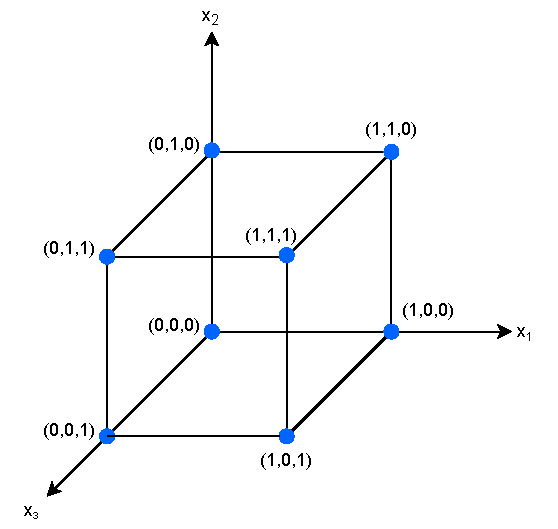
\includegraphics[scale = 0.8]{img/cubeh.pdf}
  \end{figure}
  Prendo i vertici $(x_1,x_2,x_3$):
  \begin{itemize}
    \item $(0,0,0)$
    \item $(1,0,0)$
    \item $(0,1,0)$
    \item $(0,0,1)$
    \item $(1,1,0)$
    \item $(0,1,1)$
    \item $(1,0,1)$
    \item $(1,1,1)$
  \end{itemize}
  \textit{Questi sono i nostri messaggi}.\\
  \textbf{Oltre $n=3$ farei lo stesso ma non saprei disegnarlo, avrei $n$
    lati che partono dall'origine appoggiati agli $n$ assi}.\\
  Suppongo di spedire $010$ e che si abbia un errore che porti a $110$ e sul
  cubo si nota che ci ha fatto spostare lungo un lato. \\
  Suppongo che da $010$ si arrivi a $100$, con due errori, si nota che ho due
  lati visitati sul cubo.\\
  Scegliamo quindi come messaggi validi punti che sono abbastanza distanti tra
  loro. Sicuramente quelli che si ottengono con un solo cambiamento non sono
  validi, parto quindi dal messaggio valido e impongo che tutti quelli che sono
  a \textbf{distanza 1} (parlando di \textbf{distanza di Hamming}) sul cubo,
  ovvero tutti quelli che raggiungo con un solo lato, non siano validi.\\
  \textbf{Essendo in $\{0,1\}^n$ in realtà esistono solo i vertici del cubo, i
    lati servono solo per capire meglio.}
\end{esempio}
Generalizziamo meglio.\\
Se ho la distanza di Hamming e varie caratteristiche del codice ho che:
\begin{itemize}
  \item se ho due codeword valide che hanno distanza 1 allora il codice ha
  capacità di \textbf{0 detection e 0 correction} in quanto potrei passare con
  un solo errore ad un messaggio valido
  \item se ho due codeword valide che hanno distanza 2 (e non esistono due
  codeword valide con distanza minore di 2) allora il codice ha
  capacità di \textbf{1 detection e 0 correction} in potrei avere più codeword
  valide a distanza di 1 da quella errata e quindi non saprei come fare
  correzione, non sapendo dove si trovi il bit errato. In ogni caso un errore
  viene sempre riconosciuto, anche se non può essere corretto. Se ho due errori
  potrei finire nuovamente in una codeword valida ma si sta assumendo che avendo
  scelto questo codice si sappia che la probabilità che avvengano due errori sia
  pressoché nulla. Il\textit{ controllo di parità semplice} è di questo
  tipologia.
  \newpage
  Graficamente avrei 
  una cosa del tipo, avendo in blu le codeword valide e in rosso quelle non
  valide: 
  \begin{figure}[H]
    \centering
    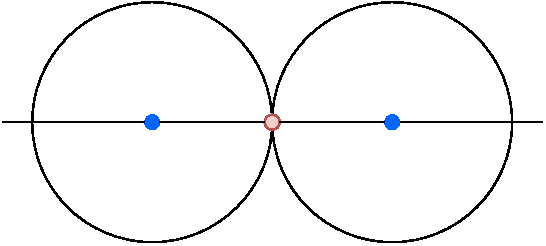
\includegraphics[scale = 0.8]{img/circ2.pdf}
  \end{figure}
  Notando come non sarei in grado di capire a che codeword valida ricondurmi.
  \item se ho due codeword valide che hanno distanza 3 (e non esistono due
  codeword valide con distanza minore di 3) allora il codice ha
  capacità di \textbf{2 detection e 1 correction}, riuscendo a correggere un
  errore. Se avessi due errori riconoscerei come codeword valida una a distanza
  1 da quella errata che però non è quella giusta, introducendo un nuovo
  errore. I \textit{codici di Hamming} sono di questo tipo. Graficamente avrei
  una cosa del tipo, avendo in blu le codeword valide e in rosso quelle non
  valide: 
  \begin{figure}[H]
    \centering
    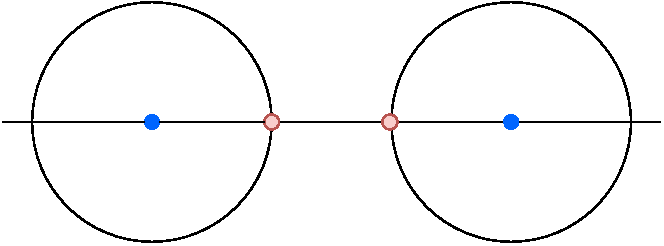
\includegraphics[scale = 0.8]{img/circ3.pdf}
  \end{figure}
  Notando che con un solo errore sarei in grado di capire a che codeword
  ricondurmi 
  \item se ho due codeword valide che hanno distanza 4 (e non esistono due
  codeword valide con distanza minore di 4) allora il codice ha
  capacità di \textbf{3 detection e 1 correction}, riuscendo a correggere un
  errore. Se avessi due errori riconoscerei avrei più codeword valide alla
  stessa distanza. Se avessi tre errori varrebbe quanto detto nel caso di
  distanza 2
   \item se ho due codeword valide che hanno distanza 5 (e non esistono due
  codeword valide con distanza minore di 5) allora il codice ha
  capacità di \textbf{4 detection e 2 correction}, per gli stessi discorsi fatti
  avendo distanza 3
\end{itemize}
Si nota quindi che al crescere della distanza di Hamming minima tra due codeword
cresce la capacità di detection e correction.\\
Possiamo ipotizzare che la codeword valida venga avvolta da una sfera di raggio
pari a $r$ avendo che $r$ sia tale per cui le sfere di due codeword valide non
si sovrappongano. Possiamo notare che in base alle osservazioni fatte sopra $r$
è il valore della capacità di detection. \\
Una sfera centrata nel punto $\vec{x}$ di raggio $r$ è l'insieme dei punti
$\vec{y}\in\{0,1\}^n$ tale che la distanza da $\vec{x}$ è minore di $r$, ovvero:
\[S(\vec{x},r)=\{\vec{y}\in\{0,1\}^n|\,d_h(\vec{x},\vec{y})\leq r\}\]
\textbf{Si noti che in $\{0,1\}^n$ somma e sottrazione bit a bit portano allo
  stesso risultato. }\\
Possiamo dire che:
\[output=input+errore\]
dove $errore$ è un vettore rappresentante l'errore (avendo $1$ dove ho
l'errore). Quindi:
\[errore = output -input\]
\begin{esempio}
  Tornando all'esempio sopra ipotizzo entri $011$ ed esca $111$, avendo quindi
  $d_h=1$. \\
  Sommo i due vettori:
  \[011\oplus 111=100\]
  Avendo che $100$ è l'errore.
\end{esempio}
\begin{esempio}
  Si vuole costruire un codice che consenta di correggere un errore, per poi
  confrontarlo con il codice di Hamming.\\
  Ci servono quindi codeword valide ad almeno distanza 3, prendendo messaggi
  validi e circondarli di sfere di raggio 1 tali che non si abbiano
  sovrapposizioni con altre sfere.\\
  Si ha $\{0,1\}^n$ come spazio vettoriale dove si hanno $2^n$
  elementi/vettori. \\
  In generale se prendo il volume dello spazio e lo divido per il volume di una
  sfera ho il numero di sfere che posso metterci:
  \[\frac{V_{spazio}}{V_{sfera}}\geq \mbox{numero massimo di sfere}\]
  Pongo $k$ uguale al numero di bit dei messaggi validi (non pari a $n$ ma
  prendo quindi una porzione di messaggio rappresentante il messaggio valido, ai
  quali poi aggiungerei le $m$ check digit).\\
  Rivedo quindi la formula, sapendo che il volume dello spazio è il numero di
  vettori di quello spazio, che le sfere abbiano raggio $1$, avendo che hanno
  volume $n+1$ (il vettore rappresentante originale più un vettore per ogni
  possibile vettore ottenuto da quello originale con un solo errore, avendo
  quindi ${{n}\choose{1}}$ più il messaggio valido, ovvero $n+1$): 
  \[\frac{2^n}{n+1}\geq 2^k\]
  sapendo che $n=k+m$ si ha che:
  \[\frac{2^{k+m}}{n+1}\geq 2^k\]
  \[\frac{2^{k}2^m}{n+1}\geq 2^k\]
  \[2^m\geq n+1\]
  Arrivando allo stesso risultato di Hamming.
\end{esempio}
Se volessi sfere di raggio maggiore di 1, prendendo per esempio con codeword
distanti almeno 5 e raggio pari a 2. Avendo raggio pari a 2 avrei il centro
della sfera, tutti i punti distanti 1, ovvero potendo cambiare due bit $n$, e
tutti i punti distanti due (avendo due 
cambiamenti di bit), ovvero:
\[V_{sfera}=1+n+{{n}\choose{2}}=1+n+\frac{n(n-1)}{2}\]
\[\frac{2^n}{1+n+\frac{n(n-1)}{2}}\geq 2^k\]
sapendo che $n=k+m$ si ha che:
\[\frac{2^{k+m}}{1+n+\frac{n(n-1)}{2}}\geq 2^k\]
\[\frac{2^{k}2^m}{1+n+\frac{n(n-1)}{2}}\geq 2^k\]
\[2^m\geq 1+n+\frac{n(n-1)}{2}\]
Avendo una generica sfera di raggio $r$ avrei:
\[V_{sfera}=1+n+{{n}\choose{2}}+{{n}\choose{3}}+\cdots+{{n}\choose{r}}=
  \sum_{k=0}^n{{n}\choose{k}}\] 
\textit{Nella realtà, con messaggi molto grandi, si usano i cosiddetti
  \textbf{low density parity codes}, che consiste, per proteggere il pacchetto
  di $n$ bit, nel trovare il minor numero di equazioni di parità atte a
  proteggere il messaggio (meno equazioni implica meno circuiti e quindi meno
  costo). Si procede per euristiche per capire quante e quali.}
\section{Codifica di Sorgente}
Finora si è parlato di \textbf{codifica di canale}, passiamo quindi ad
approfondire la \textbf{codifica di sorgente}, cercando anche in questo caso il
codice ottimale (con la lunghezza media minima).\\
Avendo magari una distribuzione non uniforme per la distribuzione dei caratteri
non ha senso usare una \textbf{codice a blocchi} ma si usa un 
\textbf{codice a lunghezza variabile} (\textit{riguardare quanto detto nella
  prima sezione di questi appunti}).\\
Ci si propone quindi di minimizzare, parlando di codici a lunghezza variabile:
\[L=\sum_{i=1}^1 p_il_i\]
Bisogna prima fare un discorso sull'univocità dei codici.
\begin{esempio}
  si supponga di avere le seguenti codeword binarie per 4 simboli $s_i$:
  \begin{itemize}
    \item $s_1\to 0$
    \item $s_2\to 01$
    \item $s_3\to 11$
    \item $s_4\to 00$
  \end{itemize}
  Suppongo che il ricevente riceva $0011$. Cerco di capire che sequenza ha
  ricevuto. Deve calcolare una:
  \[cod^{-1}:\Gamma^*\to S\]
  Ma ci sono delle ambiguità. Potrebbe essere;
  \begin{itemize}
    \item $s_4s_3$
    \item $s_1s_1s_3$
  \end{itemize}
  Non è quindi in grado di trovare una sequenza di simboli univoca.\\
  Ne segue che il codice \textbf{non è univocamente decodificabile}.
\end{esempio}
Si richiede quindi che la funzione $cod$, quindi il nostro codice, \textbf{deve
  essere univocamente decodificabile}. \\
Un algoritmo che riconosce che un codice è univocamente decodificabile non è
banale.
\begin{esempio}
  Si supponga di avere le seguenti codeword binarie per 4 simboli $s_i$:
  \begin{itemize}
    \item $s_1\to 0$
    \item $s_2\to 01$
    \item $s_3\to 011$
    \item $s_4\to 111$
  \end{itemize}
  Si dimostra che questo codice è \textbf{univocamente decodificabile},
  esistendo un'unica possibile divisione in codeword di ogni stringa che riceve
  il ricevente.\\
  Suppongo che il ricevente riceva:
  \[0111111111\]
  Ma anche solo all'inizio potrei avere sia $s_1$ che $s_2$ che $s_3$ ma una
  volta che è finito posso partire dal fondo raggruppando gli $1$ tre a tre e mi
  accorgo che ho un solo modo:
  \[0\,\,\,111\,\,\,111\,\,\,111\]
  \[s_1s_4s_4s_4\]
  \textbf{Bisogna quindi aspettare la fine della trasmissione}.
\end{esempio}
Lato elettronico per fare questa operazione uso un \textbf{contatore
  elettronico}.\\
D'altro canto aspettare la fine non è ``comodo'' e si vorrebbe analizzare i
simboli man mano che arrivano.\\
Si definiscono quindi due categorie di codici a lunghezza variabile:
\begin{itemize}
  \item \textbf{non univocamente decodificabili}
  \item \textbf{univocamente decodificabili}
\end{itemize}
e suddividiamo gli univocamente decodificabili in:
\begin{itemize}
  \item \textbf{istantaneo}, dove appena arriva una codeword il ricevente sa che
  è arrivata completamente e che è unica
  \item \textbf{non istantaneo}
\end{itemize}
\begin{esempio}
  Trasformiamo l'ultimo esempio in un codice istantaneo. Si hanno:
  \begin{itemize}
    \item $s_1\to 0$
    \item $s_2\to 01$
    \item $s_3\to 011$
    \item $s_4\to 111$
  \end{itemize}
  ma non andrebbero bene (per il problema dell'inizio del messaggio). D'altro
  canto:
   \begin{itemize}
    \item $s_1\to 0$
    \item $s_2\to 10$
    \item $s_3\to 110$
    \item $s_4\to 111$
  \end{itemize}
  ottenuto con la \textit{reverse} delle stringhe, è un codice istantaneo con
  codeword di lunghezza pari a quelle precedenti.\\
  Posso facilmente vedere che qualsiasi cosa arrivi posso capire che codeword è,
  appena l'intera codeword viene letta. Non devo aspettare l'intero messaggio ma
  al più due simboli.
\end{esempio}
Nell'esempio abbiamo usato gli $0$ come \textit{end of codeword}, infatti questo
codice è detto \textbf{comma code}, avendo che il decodificatore vede che le
codeword, tranne l'ultima, terminano per 0. Quindi o arriva uno zero terminando
la codeword o arrivano 3 uni che terminano il messaggio.\\
Potrei inoltre vedere la decodifica come un albero di
decodifica, in quanto ogni volta che arriva un simbolo posso escludere certe
codeword.
\newpage
Vediamo l'esempio relativo all'esempio precedente:
\begin{figure}[H]
  \centering
  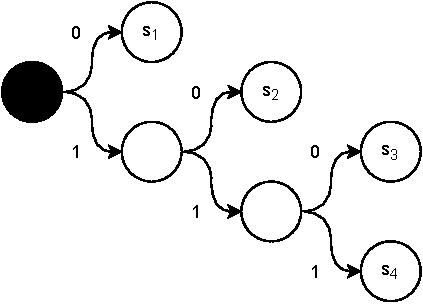
\includegraphics[scale = 0.8]{img/ct.pdf}
\end{figure}
Avendo che ogni cammino dalla radice ad una voglia è una codeword con la
foglia etichettata con il simbolo relativo alla codeword. Si ha quindi un
sottoalbero per ogni simbolo di $\Gamma$ (quindi dalla radice escono
$|\Gamma|$ archi) e da ogni nodo interno esce un numero
di archi minore o uguale al numero di simboli. Il ricevente sfrutta l'albero di
decodifica.\\ 
Posso anche usare l'albero per costruire il codice istantaneo.\\
Inoltre dato che un codice istantaneo è associato ad un albero di codifica non
succede mai che una codeword sia prefissa di un'altra (e lo si vede non prendo
avere due foglie associate a due codeword una prefissa dell'altra).
\begin{esempio}
  Vediamo l'albero di decodifica di un codice non istantaneo.\\
  Si hanno:
  \begin{itemize}
    \item $s_1\to 0$
    \item $s_2\to 01$
    \item $s_3\to 011$
    \item $s_4\to 111$
  \end{itemize}
  Si ha:
  \begin{figure}[H]
    \centering
    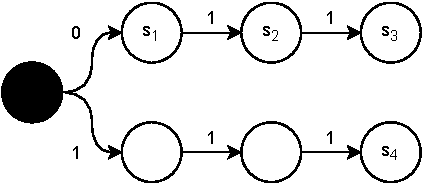
\includegraphics[scale = 0.8]{img/ct2.pdf}
  \end{figure}
  Avendo foglie che sono prefisse di altre.
\end{esempio}
Se devo costruire un codice istantaneo posso quindi usare un \textbf{comma code}
o costruire un albero di decodifica che sia il più possibile simile ad un albero
completo.
\begin{esempio}
  Si supponga di avere le seguenti codeword binarie per 5 simboli $s_i$:
  \begin{itemize}
    \item $s_1\to 0$
    \item $s_2\to 10$
    \item $s_3\to 110$
    \item $s_4\to 1110$
    \item $s_4\to 11110$
  \end{itemize}
  Si ha quindi:
   \begin{figure}[H]
    \centering
    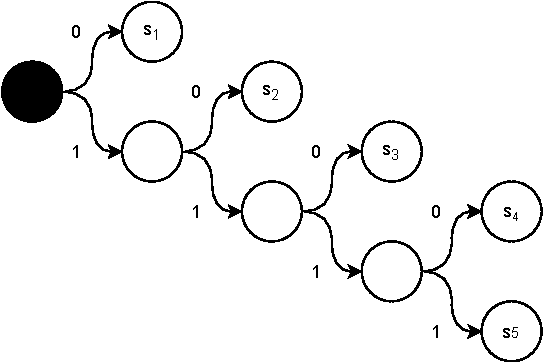
\includegraphics[scale = 0.8]{img/ct3.pdf}
  \end{figure}
  (e si nota come si possa generalizzare l'albero per un comma code).
\end{esempio}
\begin{esempio}
  Avendo l'albero:
    \begin{figure}[H]
    \centering
    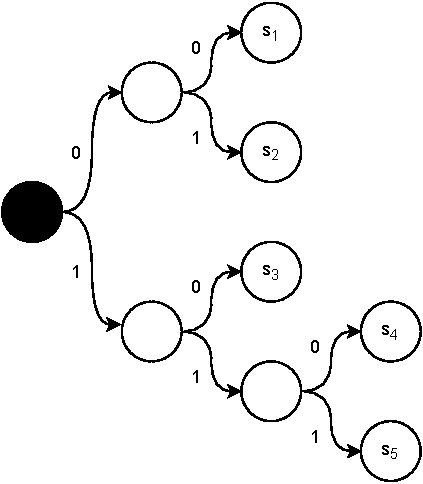
\includegraphics[scale = 0.7]{img/ct4.pdf}
  \end{figure}
  Riconosco il codice:
  \begin{itemize}
    \item $s_1\to 00$
    \item $s_2\to 01$
    \item $s_3\to 10$
    \item $s_4\to 110$
    \item $s_5\to 111$
  \end{itemize}
  
\end{esempio}
\begin{esempio}
  Avendo il codice 1:
   \begin{itemize}
    \item $s_1\to 0$
    \item $s_2\to 10$
    \item $s_3\to 110$
    \item $s_4\to 1110$
    \item $s_5\to 11110$
  \end{itemize}
  e il codice 2:
   \begin{itemize}
    \item $s_1\to 00$
    \item $s_2\to 01$
    \item $s_3\to 10$
    \item $s_4\to 110$
    \item $s_5\to 111$
  \end{itemize}
  assegno ad entrambi le probabilità:
   \begin{itemize}
    \item $p_1\to 0.9$
    \item $p_2\to 0.025$
    \item $p_3\to 0.025$
    \item $p_4\to 0.025$
    \item $p_5\to 0.025$
  \end{itemize}
  Ho che, per il primo codice:
  \[L_1=0.9\cdot 1+0.025\cdot 2+0.025\cdot 3+0.025\cdot 4+0.025\cdot 4=1.225\]
  Avendo che mediamente per rappresentare un simbolo della sorgente mi servono
  $1.225$ bit.\\
  Passo al secondo codice:
  \[L_2=0.9\cdot 2+0.025\cdot 2+0.025\cdot 2+0.025\cdot 3+0.025\cdot 3=2.05\]
  Avendo che mediamente per rappresentare un simbolo della sorgente mi servono
  $2.05$ bit.\\
  Ne segue, avendo $L_1<L_2$, per questa sorgente con queste probabilità è
  meglio il primo codice, il comma code.\\
  Se avessi avuto probabilità uniforme ($p_i=0.2$) avrei avuto:
  \[L_1=2.8\]
  \[L_2=2.4\]
  Essendo meglio il secondo codice.
\end{esempio}
\begin{definizione}
  Si definisce \textbf{codice r-ario} un codice con $r$ simboli con cui si
  ottengono le codeword.\\
  Un codice che parte da $\Gamma=\{0,1\}$ è un codice binario.
\end{definizione}
Ad un certo punto Kraft scopre un teorema che contiene una disuguaglianza che
fornisce una condizione necessaria e sufficiente affinché esista un codice
istantaneo con certe lunghezze $l_1,l_2,\ldots,l_n$ date.
\begin{teorema}[disuguaglianza di Kraft]
  Si ha che \textbf{esiste} un \textbf{codice istantaneo r-ario} per una
  sorgente $S$ di $q$ simboli, con codeword di lunghezza $l_1,l_2,\ldots,l_q$,
  sse: 
  \[\sum_{i=1}^q\frac{1}{r^{l_i}}\leq 1\]
  In onore di Kraft si ha che:
  \[K=\sum_{i=1}^q\frac{1}{r^{l_i}} \mbox{ e quindi } K\leq 1\]
  \textbf{Non si sta vedendo come sono fatte le codeword ma solo se può esistere
    un certo codice istantaneo. Sapendo che esiste poi bisogna costruire le
    codeword ma il teorema non dice nulla in merito.}\\
  La condizione necessaria e sufficiente è quindi una caratterizzazione
  dell'esistenza del codice istantaneo.
\end{teorema}
\begin{proof}
  Dobbiamo dimostrare i due versi del sse:
  \begin{enumerate}
    \item per ogni codice istantaneo r-ario di $q$ simboli con lunghezze
    $l_1,l_2,\ldots,l_q$ si ha che $K\leq 1$
    \item se $K\leq 1$ allora esiste un codice istantaneo con lunghezze
    $l_1,l_2,\ldots,l_q$ 
  \end{enumerate}
  Dimostriamo la \textbf{prima parte}.\\
  Prendo il codice e lo rappresento sull'albero di decodifica (dove ogni nodo ha
  al più $r$ archi uscenti). Ricorsivamente un albero o è vuoto o è un nodo che
  punta ad altri nodi.\\
  Parto con $r=2$, avendo codeword binarie su $\{0,1\}$ e di conseguenza alberi
  binari di decodifica. Procedo quindi con una dimostrazione per induzione sulla
  profondità dell'albero:
  \begin{itemize}
    \item \textbf{base}: profondità pari a 1. Si hanno due casi:
    \begin{enumerate}
      \item la radice o punta ad una foglia. In questo caso:
      \[K=\frac{1}{2^1}=\frac{1}{2}\leq 1\]
      \begin{figure}[H]
        \centering
        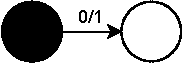
\includegraphics[scale = 0.7]{img/ct6.pdf}
      \end{figure}
      \item punta a due foglie (una per ogni simbolo). In questo caso:
      \[K=\frac{1}{2^1}+\frac{1}{2^1}=1\leq 1\]
      \begin{figure}[H]
        \centering
        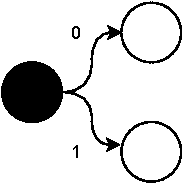
\includegraphics[scale = 0.7]{img/ct5.pdf}
      \end{figure}
    \end{enumerate}
    
    \item \textbf{passo induttivi}: assunto che il teorema è vero per ogni
    albero di profondità $n-1$ dimostriamo che il teorema vale anche per gli
    alberi di profondità $n$. In realtà così non ci va bene in quanto i
    sottoalberi dovrebbero avere entrambi profondità $n-1$ (cosa non vera come
    visto negli esempi precedenti, ad esempio ``l'\textit{albero a pettine}''
    del comma code). Cambiamo quindi dicendo che  assunto che il teorema è vero
    per ogni albero di profondità $<n$ dimostriamo che il teorema vale anche per
    gli alberi di profondità $n$.\\
    Considero i due sottoalberi come alberi a se stanti:
    \begin{figure}[H]
      \centering
      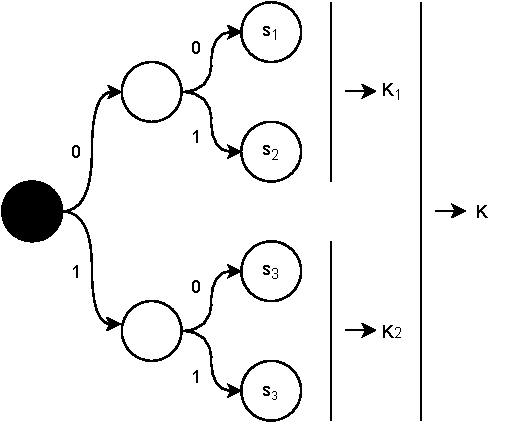
\includegraphics[scale = 0.7]{img/ct7.pdf}
    \end{figure}
    Dico che $K_1\leq 1$ per il primo sottoalbero e $K_2\leq 1$ per il secondo
    sottoalbero. \\
    Calcolo ora $K$ di tutto l'albero ma devo capire come si rapporta a $K_1$ e
    $K_2$. Si ha che se attacco il primo sottoalbero alla nuova radice per
    costruire l'albero globale ho che attacco ad ogni codeword un simbolo, che
    quindi si allungano di 1:
    \[\sum_{i=1}^q\frac{1}{r^{l_i+1}}\leq 1\]
    ma altro non è che:
    \[\sum_{i=1}^q\frac{1}{r}\cdot\frac{1}{r^{l_i}}\leq 1\]
    ma allora:
    \[\frac{1}{r}\cdot\sum_{i=1}^q\frac{1}{r^{l_i}}\leq 1=\frac{1}{r}\cdot K_1\]
    Faccio lo stesso per $K_2$ e quindi, avendo $r=2$:
    \[K=\frac{1}{2}\cdot K_1+\frac{1}{2}\cdot K_2\]
    ma sto sommando due quantità $\leq \frac{1}{2}$ (avendo $K_1\leq 1$ e
    $K_2\leq 1$) e quindi: 
    \[K\leq 1\]
  \end{itemize}
  Qualora si avesse $r>2$ si ha:
  \begin{itemize}
    \item \textbf{base}, si hanno alberi r-ari, con
    $\Gamma=\{0,1,2,\ldots,r-1\}$, di probabilità 1. Tutti questi alberi hanno
    $s$ foglie e $s-r$ non foglie. Quindi, essendo tutti gli $l_i$ uguali a 1
    essendo a profondità uno:
    \[K=\sum \frac{1}{r^{l_1}}=\sum \frac{1}{r}=\frac{s}{r}\leq 1\]
    $\frac{s}{r}\leq 1$ in quanto $s<r$
    \item \textbf{passo induttivo} si ha un albero r-ario a profondità $n$ con
    un certo numero di sottoalberi $s$ e un certo numero di sottoalberi vuoti,
    di cardinalità $s-r$, a profondità $n-1$. Per tutti i $K_1,K_2,\ldots K_s$
    ho che $K_i\leq 1$ e quindi ottengo $K$ aggiungendo un simbolo alle codeword 
    dei sottoalberi non vuoto (quelli vuoti contribuiscono con 0 alla
    sommatoria): 
    \[K=\frac{1}{r}K_1+\frac{1}{r}K_2+\cdots+\frac{1}{r}K_s\]
    Ma per lo stesso ragionamento del caso binario, essendo ogni $K_1<leq 1$ e
    quindi ogni componente della sommatoria è $\leq \frac{1}{r}$:
    \[K=\frac{1}{r}K_1+\frac{1}{r}K_2+\cdots+\frac{1}{r}K_s\leq \frac{s}{r}\leq
      1\] 
  \end{itemize}
  Vediamo la \textbf{seconda parte} della dimostrazione.\\
  Se $K\leq 1$ dobbiamo dimostrare che esiste un codice istantaneo con lunghezze
  $L_1,\ldots, l_q$.\\
  Sappiamo che:
  \[K=\sum_{i=1}^q\frac{1}{r^{l_i}}\leq 1\]
  Vediamo un esempio per capire come vedere diversamente la diseguaglianza:
  \begin{esempio}
    se avessi $r=2$, con quindi codeword binarie, e lunghezze 2,2,3,3,4 (con
    quindi $q=5$). Si ha che: 
    \[K=\frac{1}{2^2}+\frac{1}{2^2}+\frac{1}{2^3}+\frac{1}{2^3}+\frac{1}{2^4}\]
    Ma quindi:
    \[K=\frac{2}{2^2}+\frac{2}{2^3}+\frac{1}{2^4}\]
    Avendo ora 2,2,1 come numeratori.
  \end{esempio}

  Indico con $t_j$ il numero di codeword di lunghezza $j$. Si hanno quindi, per
  l'esempio precedente:
  \begin{itemize}
    \item $t_1=0$
    \item $t_2=2$
    \item $t_3=2$
    \item $t_4=1$
  \end{itemize}
  Riscrivo quindi $K$:
  \[K=\sum_{i=1}^q\frac{1}{r^{l_i}}=\sum_{j=1}^l\frac{t_j}{r^{j}}\]
  con $l=\max\{l_1,\ldots,l_q\}$ (per l'esempio sopra $l=4$).\\
  Si ha quindi che:
  \[\sum_{j=1}^l\frac{t_j}{r^{j}}\leq 1\]
  Ma posso dire che, per arrivare ad isolare i $t_j$ senza alterare la
  diseguaglianza: 
  \[r^l\cdot \sum_{j=1}^l\frac{t_j}{r^{j}}\leq 1\cdot r^l\]
  ma quindi ho che:
  \[r^l\cdot \sum_{j=1}^lt_j\cdot r^{l-j}\leq 1\cdot r^l\]
  Si ha che:
  \[ \sum_{j=1}^lt_j\cdot r^{l-j}= t_1\cdot r^{l-1}+\cdots+t_{l-1}\cdot
    r+t_l\leq r^l\]
  Ma quindi:
  \[t_l\leq r^l- t_1\cdot r^{l-1}-\cdots-t_{l-1}\cdot r\]
  ma so anche che:
  \[0\leq t_l\]
  e quindi:
  \[0\leq t_l\leq r^l- t_1\cdot r^{l-1}-\cdots-t_{l-1}\cdot r\]
  e quindi:
  \[0\leq r^l- t_1\cdot r^{l-1}-\cdots-t_{l-1}\cdot r\]
  porto quindi $t_{l-1}$ a sinistra e divido per $r$, ottenendo:
  \[t_{l-1}\leq r^{l-1}-t_1\cdot r^{l-1}-\cdots t_{l-2}\cdot r\]
  lo faccio per tutti i $t_j$ partendo da $t_{l-2}$ e arrivando a:
  \[t_2\leq r^2-t_1\cdot r\]
  sapendo per di più che:
  \[0\leq t_2\leq r^2-t_1\cdot r\]
  e poi a:
  \[0\leq t_1\leq r\]
  Risalgo quindi partendo dalle codeword più corte. Cerco $t_1$ codeword di
  lunghezza 1, avendo a disposizione l'alfabeto $\Gamma$ r-ario. Per farlo
  prendo i primi $t_1$ simboli e dico che sono le stringhe di lunghezza 1. Posso
  farlo perché $t_1\leq r$ e mi avanzano $r-t_1$ simboli dell'alfabeto.\\
  Passo alle codeword di lunghezza 2, me ne servono $t_2$. Queste codeword sono
  due simboli concatenati in modo che il primo simbolo non si stato utilizzato
  per $t_1$ (altrimenti creerei prefissi), quindi prendo un simbolo dai $r-t_1$
  simboli dell'alfabeto. Il secondo simbolo posso mettere un qualsiasi simbolo
  di $\Gamma$, avendo $r$ possibili scelte. In totale ho quindi un numero di
  combinazioni pari a:
  \[(r-t_1)\cdot r=r^2-t_1\cdot r\]
  e ho abbastanza combinazioni avendo che $t_2\leq r^2-t_1\cdot r$ per i conti
  precedenti. Le codeword le scelgo come voglio, ci sono tantissimi modi
  possibili.\\  
  Mi avanzano quindi $r^2-t_1\cdot r-t_2$.\\
  Creo le codeword di lunghezza 3 dove i primi due simboli non devono essere una
  combinazione usata per quelle di lunghezza 2, facendo poi gli stessi discorsi
  fatti sopra. \\
  Avanzo così per tutte le lunghezze di codeword avendo che posso costruire
  almeno un codice istantaneo, dimostrando la validità del teorema.
\end{proof}
\begin{esempio}
  Riprendiamo l'esempio di sopra.\\
  Si ha che: 
  \[K=\frac{1}{2^2}+\frac{1}{2^2}+\frac{1}{2^3}+\frac{1}{2^3}+\frac{1}{2^4}\]
  Ma quindi:
  \[K=\frac{2}{2^2}+\frac{2}{2^3}+\frac{1}{2^4}=\frac{3}{4}+\frac{1}{16}\leq 1\]
  \newpage
  Se volessi le codeword costruisco l'albero di decodifica:
  \begin{figure}[H]
    \centering
    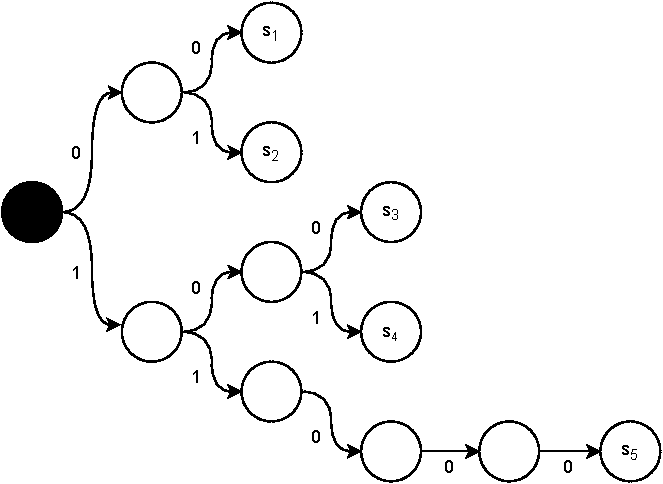
\includegraphics[scale = 0.7]{img/ct8.pdf}
  \end{figure}
  Avendo:
   \begin{itemize}
    \item $s_1\to 00$
    \item $s_2\to 01$
    \item $s_3\to 100$
    \item $s_4\to 101$
    \item $s_5\to 1100$
  \end{itemize}
  Ma vedo che ho nodi interni inutili (tipo i due nodi che portano a $s_5$).
  Butto via quindi i nodi con un solo ramo in uscita:
  \begin{figure}[H]
    \centering
    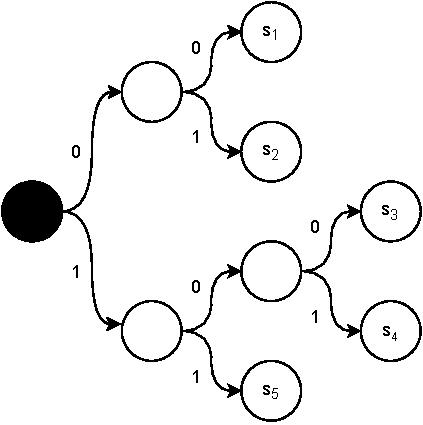
\includegraphics[scale = 0.7]{img/ct9.pdf}
  \end{figure}
  ottenendo:
  \begin{itemize}
    \item $s_1\to 00$
    \item $s_2\to 01$
    \item $s_3\to 100$
    \item $s_4\to 101$
    \item $s_5\to 11$
  \end{itemize}
  e quindi:
  \[K=\frac{3}{2^2}+\frac{2}{2^3}=\frac{3}{4}+\frac{1}{4}=1\leq 1\]
\end{esempio}
Quindi un nodo interno che solo un figlio mi fa allungare le lunghezze delle
codeword facendo sommare valori più piccoli. Se ho solo nodi interni con due
figli si può dimostrare per induzione che $K=1$ (nel caso base ho $K=1$ e in
quello induttivo vedo che ho $K_i=1$ per ogni sottoalbero, avendo poi che
$K=\frac{1}{2}K_1+\frac{1}{2}K_2=\frac{1}{2}\cdot 1+\frac{1}{2}\cdot 1= 1$).\\
Per tutti i codici istantanei vale che $K\leq 1$.
\subsection{Codici a Blocchi Accorciati}
Si vuole costruire un codice binario per un certo $q$.
\begin{esempio}
  Ipotizzo $r=2$ e
  $q=5$. Potrei avere tutte le 8 codeword di 3 bit ma ne scelgo solo $5$. Tengo
  $000,010,100,110,111$, avendo rimosso $001,011,101$. Queste 5 formano un
  codice a blocchi, istantaneo. Potrebbe non essere efficiente, non avendo
  $K=1$. Se costruissi l'albero avrei:
  \begin{figure}[H]
    \centering
    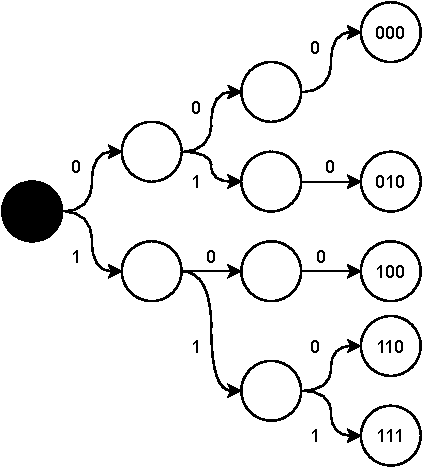
\includegraphics[scale = 0.7]{img/b.pdf}
  \end{figure}
  Che ha $K\neq 1$.
  \newpage
  Potrei rimuovere archi inutili, ottenendo:
  \begin{figure}[H]
    \centering
    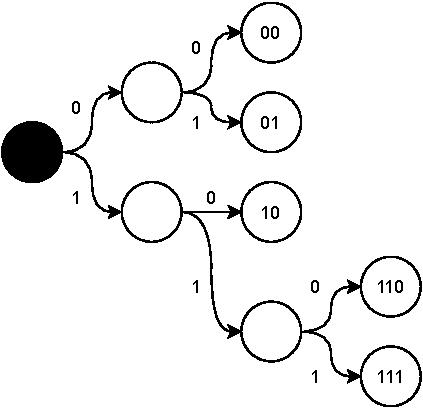
\includegraphics[scale = 0.7]{img/b2.pdf}
  \end{figure}
  Ottenendo:
  \begin{itemize}
    \item 00
    \item 01
    \item 10
    \item 110
    \item 111
  \end{itemize}
  Che non è più a blocchi ma è istantaneo con $K=1$ (ogni nodo interno ha
  infatti esattamente due figli).
\end{esempio}
Si sta parlando appunto di \textbf{codici a blocchi accorciati}.\\
\textbf{Su file esercizi esempio con codice non binario}.
\subsection{Disuguaglianza di McMillan}
\begin{teorema}[Disuguaglianza di McMillan]
  Data una sorgente $S=\{s_1,\ldots,s_q\}$ si ha che una condizione necessaria e
  sufficiente affinché esista un codice r-ario univocamente decodificabile con
  codeword di lunghezze $l_1,l\dots,l_q$ è che valga:
  \[K=\sum_{i=1}^q\frac{1}{r^{l_1}}\leq 1\]
  \textup{Quindi è uguale alla disuguaglianza di Kraft semplicemente sostituendo
  ``codici istantanei'' con ``codice univocamente decodificabile''.}
\end{teorema}
\begin{proof}
  Anche in questo caso si hanno i due versi della dimostrazione.\\
  La \textbf{prima parte} è dimostrare che dato un codice r-ario per $S$
  univocamente decodificabile allora $K\leq 1$ e per tale codice le lunghezze
  sono $l_1,l\dots,l_q$. Il ``dato'' è in realtà un ``per ogni''.\\
  Non posso più ragionare sulla profondità dell'albero non avendo più
  corrispondenza biunivoca con alberi dove le codeword sono le foglie. In questo
  caso avrei nodi interni che sono codeword, non posso quindi usare la stessa
  tecnica di dimostrazione.\\
  Per dimostrarlo prendo $K$ e un numero $n\in\mathbb{N}$, tale che
  $n>1$. Calcolo $K^n$, avendo:
  \[K^n=\left(\sum_{i=1}^q\frac{1}{r^{l_1}}\right)^n\]
  Ottenendo qualcosa di davvero difficile da studiare. Ma posso scrivere:
  \[K^n=\sum_{t=n}^{n\cdot l}\frac{n_t}{r^{t}}\]
  indicando con $n_t$ il numero di termini con $t$ (??? risentire) e con
  $l=\max\{l_1,\ldots,l_q\}$. Si ha che $n_t$ è anche il numero di codeword di
  lunghezza $t$. Ma dato che il codice è univocamente decodificabile si ha che:
  \[n_t\leq r^t\]
  ma allora:
  \[\frac{n_t}{r^{t}}\leq 1\]
  Ma allora si può dire, maggiorando, che:
  \[K^n=\sum_{t=n}^{n\cdot l}\frac{n_t}{r^{t}}\leq \sum_{t=n}^{n\cdot
      l}1=n\cdot l-n+1=n\cdot l-(n-1)\]
  Ma $(n-1)>0$ e quindi:
  \[=n\cdot l-(n-1) < n\cdot l\]
  E quindi:
  \[K^n<n\cdot l\]
  \newpage
  Questo si risolve graficamente (\textbf{grafico molto approssimato}):
  \begin{figure}[H]
    \centering
    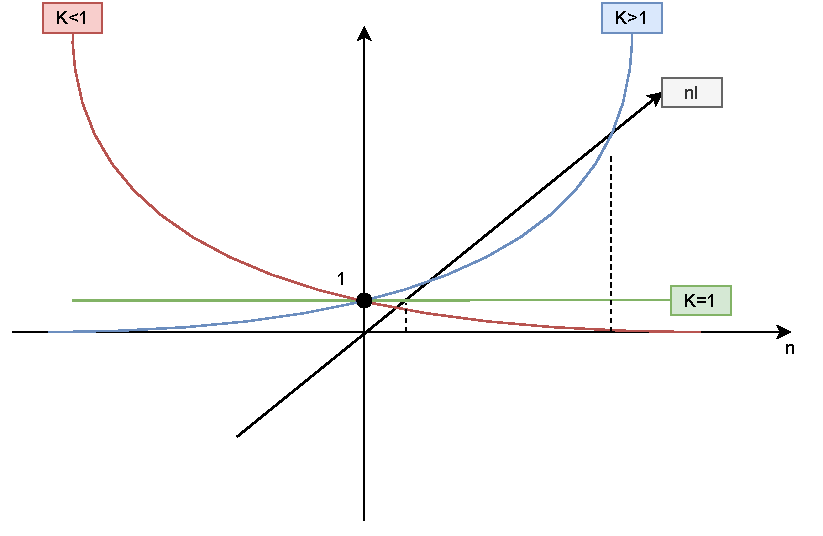
\includegraphics[scale = 0.8]{img/grap.pdf}
  \end{figure}
  Se $K>1$ ad un certo punto la curva supera $n\cdot l$. Per $K<1$ sicuramente
  ho punti per cui è $<n\cdot l$ e quindi si arriva a dire che:
  \[K^n<n\cdot l\implies K\leq 1\]
  dimostrando la tesi.\\
  
  La \textbf{seconda parte} è che se $K\leq 1$ allora esiste un codice r-ario
  per $S$ univocamente decodificabile con lunghezze $l_1,l\dots,l_q$. Per Kraft,
  avendo $K\leq 1$ esiste un codice istantaneo per $S$, r-ario, con tali
  lunghezze. Ma \textbf{un codice istantaneo è univocamente decodificabile},
  avendo quindi dimostrato la tesi.
\end{proof}
Ma avendo che i codici univocamente decodificabili sono meno utili di quelli
istantanei vengono trascurati, considerando che dovrei fare la ``stessa
fatica''.\\
Abbiamo visto comunque che non si hanno indicazioni in merito a come fare le
codeword e abbiamo anche trascurato finora l'uso delle probabilità.
\subsection{Codici di Huffman}
I codici di Huffman sono ottimali, ovvero raggiungono il minimo valore possibile
della lunghezza media $L$:
\[L=\sum_{i=1}^q p_i\cdot l_i\]
\begin{teorema}
  In input abbiamo quindi il codice $S$, con $s_i,\ldots s_q$, con probabilità
  $p_1,\ldots, p_q$. Il codice di Huffman ci restituisce in output sia le
  lunghezze $l_i$ che le codeword $\gamma_i$.\\
  Bisogna prima fare qualche ragionamento.\\
  Si supponga di avere i simboli in ordine di probabilità, avendo:
  \[p_1\leq p_2\leq \cdots\leq p_q\]
  ma quindi si ha che:
  \[l_1\leq l_2\leq \cdots \leq l_q\]
  perché altrimenti non avrei il codice ottimale.
\end{teorema}
\begin{proof}
  Si supponga infatti di avere
  $p_m>p_n$ e $l_m>l_n$. Studio quindi il contributo dei due simboli:
  \[p_m\cdot l_m+p_n\cdot l_n\]
  Scambio in modo che $p_m$ riceva la codeword $l_n$:
  \[p_m\cdot l_n+p_n\cdot l_m\]
  Faccio la differenza:
  \[(p_m\cdot l_n+p_n\cdot l_m)-(p_m\cdot l_m+p_n\cdot l_m)\]
  \[=p_m\cdot (l_n-l_m)-p_n\cdot (l_n-l_m)\]
  \[=(p_m-p_n)\cdot(l_n-l_m)\]
  Ma abbiamo che $p_m>p_n$ e quindi $(p_m-p_n)>0$ e per lo stesso ragionamento,
  avendo $l_m>l_n$, $(l_n-l_m)<0$. Si ha quindi che:
  \[(p_m\cdot l_n+p_n\cdot l_m)-(p_m\cdot l_m+p_n\cdot l_m)<0\]
  e quindi:
  \[p_m\cdot l_n+p_n\cdot l_m<[p_m\cdot l_m+p_n\cdot l_n\]
  perdendo quindi l'ottimalità del codice. 
\end{proof}
Deve quindi valere:
\[p_1\leq p_2\leq \cdots\leq p_q\]
e
\[l_1\leq l_2\leq \cdots \leq l_q\]
Si ha quindi un algoritmo greedy per ottimizzare la lunghezza media. Non
sappiamo se si ha un matroide ma si vedrà che tale algoritmo porta
all'ottimo. Vediamo in primis un esempio.
\begin{esempio}
  Vediamo un esempio di questo algoritmo:\\
  Presa una sorgente con $5$ simboli con le annesse probabilità (sono già
  ordinati): 
  \begin{itemize}
    \item $s_1$ con $p_1=0.4$
    \item $s_2$ con $p_2=0.2$
    \item $s_3$ con $p_3=0.2$
    \item $s_4$ con $p_4=0.1$
    \item $s_5$ con $p_5=0.1$
  \end{itemize}
  Si assuma $r=2$.\\
  Prendo i due simboli meno probabili e li unisco creando un nuovo simbolo
  ``fittizio'' con probabilità pari alla somma dei due (nel nostro caso quindi
  $0.1+0.1=0.2$). Si ha quindi, mantenendo sempre l'ordine (metto il simbolo
  combinato in coda a parità di probabilità):
  \begin{itemize}
    \item $s_1$ con $p_1=0.4$
    \item $s_2$ con $p_2=0.2$
    \item $s_3$ con $p_3=0.2$
    \item $s_{4,5}$ con $p_{4,5}=0.2$
  \end{itemize}
  Avendo ora una nuova sorgente di 4 simboli (quindi ipoteticamente più semplice
  da codificare di quella da $5$).\\
  Itero facendo la stessa cosa:
  \begin{itemize}
    \item $s_1$ con $p_1=0.4$
    \item $s_{3,4,5}$ con $p_{3,4,5}=0.4$
    \item $s_2$ con $p_2=0.2$
  \end{itemize}
  Avendo ora 3 simboli. Proseguo:
  \begin{itemize}
    \item $s_{2,3,4,5}$ con $p_{2,3,4,5}=0.6$
    \item $s_1$ con $p_1=0.4$
  \end{itemize}
  Che è facile da codificare, associando 0 e 1 (l'ordine è opzionale):
  \begin{itemize}
    \item $s_{2,3,4,5}$ con $p_{2,3,4,5}=0.6$: 0
    \item $s_1$ con $p_1=0.4$: 1
  \end{itemize}
  Costruisco quindi la sorgente a 3 (usando 0 come prefisso di tutti i nuovi):
  \begin{itemize}
    \item $s_1$ con $p_1=0.4$: 1
    \item $s_{3,4,5}$ con $p_{3,4,5}=0.4$: 00
    \item $s_2$ con $p_2=0.2$: 01 (infatti 10 non andrebbe bene avendo 1 come prefisso)
  \end{itemize}
  proseguo (usando 00 come prefisso di tutti i nuovi):
    \begin{itemize}
    \item $s_1$ con $p_1=0.4$: 1
    \item $s_2$ con $p_2=0.2$: 01
    \item $s_3$ con $p_3=0.2$: 000
    \item $s_{4,5}$ con $p_{4,5}=0.2$: 001
  \end{itemize}
  termino con lo stesso ragionamento (avendo ora 001 come prefisso):
  \begin{itemize}
    \item $s_1$ con $p_1=0.4$: 1
    \item $s_2$ con $p_2=0.2$: 01
    \item $s_3$ con $p_3=0.2$: 000
    \item $s_4$ con $p_4=0.1$: 0010
    \item $s_5$ con $p_5=0.1$: 0011
  \end{itemize}
  Che ha:
  \[L=0.4\cdot 1+0.2\cdot 2+0.2\cdot 3+0.1\cdot 4+0.1\cdot 4 =
    2.2\frac{bit}{simbolo}\]
  Se invece metto i nuovi simboli più in alto possibile avrei:
  \begin{itemize}
    \item $s_1$ con $p_1=0.4$
    \item $s_{4,5}$ con $p_{4,5}=0.2$
    \item $s_2$ con $p_2=0.2$
    \item $s_3$ con $p_3=0.2$
  \end{itemize}
  e quindi:

  \begin{itemize}
    \item $s_{2,3}$ con $p_{2,3}=0.4$
    \item $s_1$ con $p_1=0.4$
    \item $s_{4,5}$ con $p_{4,5}=0.2$
  \end{itemize}
  e quindi:

  \begin{itemize}
    \item $s_{1,4,5}$ con $p_{1,4,5}=0.6$
    \item $s_{2,3}$ con $p_{2,3}=0.4$
  \end{itemize}
  Procedendo come nel caso precedente sopra si avrebbe (\textbf{verificare i
    passaggi}): 
   \begin{itemize}
    \item $s_{1,4,5}$ con $p_{1,4,5}=0.6$: 0
    \item $s_{2,3}$ con $p_{2,3}=0.4$: 1
  \end{itemize}
  e quindi:
  \begin{itemize}
    \item $s_{2,3}$ con $p_{2,3}=0.4$: 1
    \item $s_1$ con $p_1=0.4$: 00
    \item $s_{4,5}$ con $p_{4,5}=0.2$: 01
  \end{itemize}
  e quindi:
  \begin{itemize}
    \item $s_1$ con $p_1=0.4$: 1
    \item $s_{4,5}$ con $p_{4,5}=0.2$: 01
    \item $s_2$ con $p_2=0.2$: 000
    \item $s_3$ con $p_3=0.2$: 001
  \end{itemize}
  e infine:
  \begin{itemize}
    \item $s_1$ con $p_1=0.4$: 00
    \item $s_2$ con $p_2=0.2$: 10
    \item $s_3$ con $p_3=0.2$: 11
    \item $s_4$ con $p_4=0.1$: 010
    \item $s_5$ con $p_5=0.1$: 011
  \end{itemize}
  Che ha:
  \[L=0.4\cdot 2+0.2\cdot 2+0.2\cdot 2+0.1\cdot 3+0.1\cdot 3 =
    2.2\frac{bit}{simbolo}\]
  che è uguale a prima.
\end{esempio}
\textit{Questo algoritmo greedy funziona, producendo l'ottimo, quando
  sottostante al problema si ha un matroide.}
\begin{teorema}
  Si può dimostrare che non cambia nulla, in termini di lunghezza media,
  mettendo il nuovo simbolo il più in alto/basso possibile, a parità di
  probabilità.\\
  Si può anche
  dimostrare che se metto il simbolo combinato in basso aumenta la varianza tra
  le codeword (avendo codeword di lunghezza più ``distante'') mentre mettendoli
  più in alto possibile si diminuisce la varianza. SI ricorda che la varianza è:
  \[V=\sum_{i=1}^q p_i\cdot (l_i-L)^2\]
\end{teorema}
\textbf{Esempi sul file di esercizi}.\\
\textit{Solitamente comunque si preferisce abbassare la varianza tenendo quindi
  il nuovo simbolo più in alto possibile.}
\begin{teorema}
  Il codice di Huffman è ottimo, avendo la minor lunghezza media. In altri
  termini produce codici istantanei ottimali.
\end{teorema}
\begin{proof}
  Si procede per assurdo.\\
  Si ricorda che le lunghezza vengono conosciute solo a fine algoritmo di
  calcolo.\\ 
  Supponiamo, data una sorgente $S$ con $q$ simboli $s_1,\ldots,s_q$, con
  $p_1,\ldots, p_q$, che $l_1,\ldots, l_q$ siano le lunghezze di Huffman, avendo
  quindi in corrispondenza $L_H$, lunghezza di Huffman, come:
  \[L_H=\sum_{i=1}^q p_i\cdot l_i\]
  Se non fosse ottimo avremmo un altro codice con una migliore lunghezza media
  $L'$, tale che $L'< L_H$. Entrambi sono codici istantanei con associati i due
  alberi di decodifica. Prendo quindi i due simboli meno probabili (che sono
  anche i più lunghi) per il codice di Huffman: $s_q$ e $s_{q-1}$. Si potrebbe
  dimostrare che la lunghezza delle due codeword più lunghe è uguale. Questi due
  simboli sono presi, a parità di probabilità, in modo che condividano il nodo
  genitore nell'albero. Si ha che $l_q=l_{q-1}$, condividendo il genitore e non
  avendo nodi ``sprecati'' nell'albero di decodifica.\\
  Collasso questi due nodi e il genitore in un solo simbolo fittizio che tiene
  conto di entrambi i simboli. In pratica faccio uno dei ``passi in avanti''
  dell'algoritmo sopra specificato per il calcolo dei codici di Huffman. La
  lunghezza decresce di una certa quantità $x$. Si ha in partenza che
  $p_{q-1}\cdot l_{q-1}+p_q\cdot l_q=l_q\cdot (p_{q-1}+p_q)$. Il nuovo simbolo
  avrà:
  \[(l_q-1)\cdot (p_{q-1}+p_q)=l_q\cdot (p_{q-1}+p_q)- (p_{q-1}+p_q)\]
  ovvero la stessa quantità di prima meno $(p_{q-1}+p_q)$. Quindi dalla
  lunghezza media tiro via questa quantità, ovvero $x=(p_{q-1}+p_q)$.\\
  Se vogliamo minimizzare la lunghezza media il simbolo con $p_i$ più alta ha
  $l_i$ più bassa (come dimostrato precedentemente).\\
  Faccio lo stesso ragionamento nell'altro codice (che suppongo per assurdo
  migliore di quello di Huffman e quindi essendo ottimale vale lo stesso
  rapporto tra $p_i$ e $l_i$), prendendo $s_q'$ e
  $s_{q-1}'$ (che sono quelli con probabilità minore, lunghezza maggiore nel
  secondo codice e lunghezza uguale), fondendoli in un nuovo simbolo
  fittizio, facendo gli stessi ragionamento fatto per il codice di Huffman.
  Si ha in partenza che $p_{q-1}\cdot l_{q-1}+p_q\cdot l_q=l_q\cdot
  (p_{q-1}+p_q)$.  
  Il nuovo simbolo avrà:
  \[(l_q-1)\cdot (p_{q-1}+p_q)=l_q\cdot (p_{q-1}+p_q)- (p_{q-1}+p_q)\]
  La riduzione della lunghezza quindi è la stessa che nel caso di Huffman 
  $L_H-x$ e $L'-x$.\\ 
  Si stanno ``collassando'' gli stessi simboli e le lunghezze medie decrescono
  della stessa quantità.\\
  Ad un certo punto da entrambe le parti si arriva ad avere due
  simboli. Nell'albero si avranno quindi la radice e due simboli fittizi. Per il
  secondo codice si avrà comunque una sorgente con due figli e basta. \\
  Per Huffman so che ho due codeword di lunghezza 1 (un ramo con 0 e uno con 1)
  e quindi $L_h=1$ ma sotto questo valore non posso andare, non posso codificare
  due codeword che mi portino ad una lunghezza media $<1$ per il secondo codice
  che quindi ha lunghezza media pari a $1$. Si è dimostrato che l'assurdo è
  impossibile e quindi l'algoritmo di Huffman produce codici ottimali.
\end{proof}
\subsubsection{Codici di Huffman r-ari}
Vediamo ora i codici di Huffman per $r>2$.\\
\begin{esempio}
  Vogliamo un codice r-ario con $r=4$ e quindi $\Gamma=\{0,1,2,3\}$ con una
  sorgente di $q=8$ simboli. Si hanno le seguenti probabilità:
  \begin{itemize}
    \item $p_0=0.22$
    \item $p_1=0.20$
    \item $p_2=0.28$
    \item $p_3=0.15$
    \item $p_4=0.10$
    \item $p_5=0.08$
    \item $p_6=0.05$
    \item $p_7=0.02$
  \end{itemize}
  In questo caso non fondo gli ultimi due simboli ma gli ultimi 4. Al primo
  passo ottengo:
  \begin{itemize}
    \item $p_{4,5,6,7}=0.25$
    \item $p_0=0.20$
    \item $p_1=0.28$
    \item $p_2=0.15$
    \item $p_3=0.10$
  \end{itemize}
  e poi:
  \begin{itemize}
    \item $p_{0,1,2,3}=0.75$
    \item $p_{4,5,6,7}=0.25$
  \end{itemize}
  Associo 0 e 1:
    \begin{itemize}
    \item $p_{0,1,2,3}=0.75$: 0
    \item $p_{4,5,6,7}=0.25$: 1 
  \end{itemize}
  ricostruisco usando tutti e 4 i simboli:
    \begin{itemize}
    \item $p_{4,5,6,7}=0.25$: 1
    \item $p_0=0.20$: 00
    \item $p_1=0.28$: 01
    \item $p_2=0.15$: 02
    \item $p_3=0.10$: 03
  \end{itemize}
  e infine:
  \begin{itemize}
    \item $p_0=0.22$: 00
    \item $p_1=0.20$: 01
    \item $p_2=0.28$: 02
    \item $p_3=0.15$: 03
    \item $p_4=0.10$: 10
    \item $p_5=0.08$: 11
    \item $p_6=0.05$: 12
    \item $p_7=0.02$: 13
  \end{itemize}
  \textbf{Ma questo non è ottimale}, infatti potrei dire che $13$ è 2 e che $12$
  è $3$ che non sono prefissi, per esempio. Questo succede perché nell'ultimo
  step ho usato solo 0 e 1 e non tutti i simboli possibili della sorgente,
  perdendo diverse codeword. Voglio quindi arrivare all'ultimo step con
  esattamente 4 simboli. Per farlo aggiungo simboli fittizi alla sorgente in
  modo che raccogliendo a botte di $r$ si arrivi alla fine con $r$ simboli.\\
  Si ha ad esempio:
  \begin{itemize}
    \item $p_0=0.22$
    \item $p_1=0.20$
    \item $p_2=0.28$
    \item $p_3=0.15$
    \item $p_4=0.10$
    \item $p_5=0.08$
    \item $p_6=0.05$
    \item $p_7=0.02$
    \item $p_8=0$
    \item $p_9=0$
  \end{itemize}
  Al primo passo ottengo:
  \begin{itemize}
    \item $p_0=0.22$
    \item $p_1=0.20$
    \item $p_2=0.28$
    \item $p_3=0.15$
    \item $p_4=0.10$
    \item $p_5=0.08$
    \item $p_{6,7,8,9}=0.07$
  \end{itemize}
  e poi:
  \begin{itemize}
    \item $p_{3,4,5,6,7,8,9}=0.40$
    \item $p_0=0.22$
    \item $p_1=0.20$
    \item $p_2=0.28$
  \end{itemize}
  associo quindi i simboli:
   \begin{itemize}
    \item $p_{3,4,5,6,7,8,9}=0.40$: 0
    \item $p_0=0.22$: 1
    \item $p_1=0.20$: 2
    \item $p_2=0.28$: 3
  \end{itemize}
  avendo:
  \begin{itemize}
    \item $p_0=0.22$: 1
    \item $p_1=0.20$: 2
    \item $p_2=0.28$: 3
    \item $p_3=0.15$: 00
    \item $p_4=0.10$: 01
    \item $p_5=0.08$: 02
    \item $p_{6,7,8,9}=0.07$: 03
  \end{itemize}
  e quindi:
  \begin{itemize}
    \item $p_0=0.22$: 1
    \item $p_1=0.20$: 2 
    \item $p_2=0.28$: 3
    \item $p_3=0.15$: 00
    \item $p_4=0.10$: 01
    \item $p_5=0.08$: 02
    \item $p_6=0.05$: 030
    \item $p_7=0.02$: 031
    \item $p_8=0$: 032
    \item $p_9=0$: 033
  \end{itemize}
  Ma le ultime due non mi servono:
  \begin{itemize}
    \item $p_0=0.22$: 1
    \item $p_1=0.20$: 2 
    \item $p_2=0.28$: 3
    \item $p_3=0.15$: 00
    \item $p_4=0.10$: 01
    \item $p_5=0.08$: 02
    \item $p_6=0.05$: 030
    \item $p_7=0.02$: 031
  \end{itemize}
  \textbf{Che è ottimale}.\\
  Si può calcolare che:
  \[L=1.47\,\,\,simboli\,\,\, quaternari\]
\end{esempio}
Si dimostra che si ottengono con questo processo codici ottimali e si dimostra
in modo analogo al caso binario con $r=2$ (avendo che si ragiona non con due
figli ma con $r$ figli).\\
Capiamo meglio quanti simboli fittizi con probabilità nulla vanno aggiunti.
Avendo $q$ simboli mi serve un numero, che sia il minore possibile, $q'$ di
simboli tale che $q'\geq q$. Devo quindi aggiungere $q'-q$ simboli fittizi con
probabilità 0. In ogni passo tolgo $r$ simboli e ne aggiungo 1, quindi ne tolgo
$r-1$. Partendo da $q'$ diventano poi $q'-(r-1)$ e poi $q'-(r-1)-(r-1)$ e così
via. Alla fine voglio che ne restino $r$. Partendo dal fondo ho $r+(r-1)$ poi
$(r+2\cdot (r-1))$ etc$\ldots$ Si ha quindi che, per un certo $k$:
\[q'=k\cdot(r-1)+r\]
Ma posso togliere il numero $K$ di passi:
\[q'=(k+1)\cdot (r-1)+1\to q' \equiv 1\bmod (r-1)\]
Quindi devo trovare il più piccolo $q'\geq q$ tale che $q'$ è congruo a $1\bmod
(r-1)$. Al massimo dovrò mettere $r-1$ simboli fittizi.
\begin{shaded}
  Si ricorda che:
  \[a\equiv b\bmod n\iff \exists z\in\mathbb{Z}\mbox{ t.c. }a-b=z\cdot n\]
\end{shaded}
\begin{esempio}
  Nell'esempio sopra avevamo $q=8$ e $r=4$. Mi serve $q'\geq 8$ tale che $q'$ è
  congruo a $1\bmod 3$. I primi numeri congrui a $1\bmod 3$ sono:
  \[\{1,4,7,10\}\]
  e il più piccolo $\geq 8$ è 10 e quindi $q'=10$ e quindi $q'-q=2$. 
\end{esempio}
\textbf{Per $r=2$ facendo i conti si vede che arrivo sempre ad avere sempre e
  solo due simboli nell'ultimo passaggio}.\\
Si nota che posso codificare le cifre quaternarie tramite quelle binarie, $0\to
00$, $1\to 01$, $2\to 10$ e $3\to 11$, passando da uno a due simboli,
raddoppiando quindi anche le lunghezze delle codeword e il doppio della
lunghezza media, raggiungendo però un codice non ottimale (applicando
direttamente l'algoritmo di Huffman con $r=2$ si può dimostrare si ottiene un
codice migliore, avendo codeword di lunghezza due e tre e non due e quattro).\\
\begin{algorithm}
  \begin{algorithmic}
    \Function{Huffman}{$S=\{s_1,s_2,\ldots,s_n\},\,\,\, F$}
    \State $Q\gets \emptyset$
    \State \textit{inserire tutti gli} $s_i$ \textit{in} $Q$
    \For{$i\gets 1$ \textbf{to} $|S|$}
    \State \textit{alloca un nodo} $n$
    \State $left[n]\gets x\gets\mbox{extract\_min(Q)}$
    \State $right[n]\gets y\gets \mbox{extract\_min(Q)}$
    \State $F(n)\gets F(x)+F(z)$
    \State $Q.insert(n)$
    \EndFor
    \EndFunction
  \end{algorithmic}
  \caption{Pseudocodice dell'algoritmo di Huffman, con $S$ insieme dei simboli,
  $F$ che associa una frequenza ad ogni simbolo, $Q$ coda di priorità. Il codice
  non è stato trattato in aula ma mi sembrava interessante averlo.}
\end{algorithm}
Finora le sorgenti funzionavano che ad ogni colpo di clock uscisse un simbolo,
con probabilità associata, ignorando quanto successo prima. Si ha quindi che
queste sorgenti sono \textbf{memoryless}. 
\begin{definizione}
  Definiamo una \textbf{sorgente con memoria}.\\
  SU supponga di avere una memoria di ordine $j$. Si ha che il simbolo $s_i$
  esce con probabilità:
  \[p(s_i|s_{i1},s_{i2},\ldots,s_{ij})\]
  in pratica la probabilità di un simbolo è condizionata dai $j$ simboli usciti
  precedentemente. Questa è una sorgente con memoria.\\
  Il loro studio avviene tramite \textbf{processi di Markov} e
  \textbf{matrici}.\\
  Si cerca una distribuzione di probabilità, espressa tramite vettore, $\pi$
  tale che $\pi=M\pi$, con $M$ matrice. Si vuole quindi che ciascun simbolo esce
  con la probabilità indicata nel vettore $\pi$ in modo che sia un \textbf{punto
    fisso} (???). \\
  \textbf{\textit{Spiegazione superficiale in quanto al tematica non viene
      approfondita.}} 
\end{definizione}
L'algoritmo di Huffman si può adattare alle sorgenti con memoria.
\section{L'informazione}
Si ha sempre una sorgente $S$ senza memoria con i simboli $s_i$ a cui sono
associate le probabilità $p_i$. Cerchiamo di capire quanta informazione ci dà un
simbolo:
\[I(s_i)=?\]
L'informazione dipende soprattutto dal destinatario, da quanto è in grado di
comprendere tale informazione. Cambiare ricevente cambia tale valore.\\
Si arriverà a capire quanto si può comprimere un messaggio tramite la quantità
di informazione ma studiando solo dal punto di vista del messaggio ignorando il
ricevente.\\
Studiamo il rapporto tra $p_i$ e $I(s_i)$. Shannon dice che eventi più rari
forniscono una maggior quantità di informazione, essendo inversamente
proporzionale: 
\[I(s_i)=\frac{1}{p_i}\]
Si vuole anche che da due sottosistemi che producono due quantità di
informazioni $I(A)$ e $I(B)$ si possa ottenere l'informazione totale del
sistema $C$. Si vuole che valga l'additività:
\[I(C)=I(A)+I(B)\]
In realtà possiamo dire che che $I$ prende in input la probabilità stessa,
avendo:
\[I(p_i)=\frac{1}{p_i}\]
Se ho a che fare con due eventi indipendenti ho che:
\[I(p_i\cdot p_j)=\frac{1}{p_i\cdot p_j}\]
ma ho che $[I(p_i)=\frac{1}{p_i}$ e $I(p_j)=\frac{1}{p_j}$ e quindi vorrei:
\[I(p_i\cdot p_j)=\frac{1}{p_i\cdot
    p_j}=\frac{1}{p_i}+\frac{1}{p_j}=\frac{p_i+p_j}{p_i\cdot p_j}\neq
  \frac{1}{p_i\cdot p_j}\]
e quindi non va bene.\\
Ma l'additività la hanno potenze e logaritmi, quindi si dice che:
\[I(p_i)=\log_2\frac{1}{p_i}\]
Ma quindi:
\[I(p_i\cdot p_j)=\log_2\frac{1}{p_i\cdot
    p_j}=\log_2\left(\frac{1}{p_i}\cdot\frac{1}{p_j}\right)=
  \log_2\frac{1}{p_i}+\log_2\frac{1}{p_j}=I(p_i)+I(p_j)\]
Dal punto di vista assiomatico chiediamo che la quantità di informazione goda di
queste proprietà, avendo $I:[0,1]\to\mathbb{R}_0^+$:
\begin{itemize}
  \item $I(p)>0$
  \item $I(p_1\cdot p_2)=I(p_1)+I(p_2)$ se gli eventi sono indipendenti, valendo
  l'additività 
  \item $I(p)$ è una funzione continua, per non avere situazioni scomode
\end{itemize}
Già solo con queste proprietà se ne ricavano altre:
\begin{itemize}
  \item $I(P^n)=n\cdot I(p),\forall n\in \mathbb{N}$ e si potrebbe dimostrare
  per induzione. $I(P^1)=1\cdot I(P)$ e \[I(p^n)=I(p^{n-1}\cdot
    p)=I(P^{n-1})+I(p)=I(p)+(n-1)\cdot I(p)=n\cdot I(p)\]
  \item $y=p^n\to p=y^{\frac{1}{n}}$ e quindi:
  \[I(y)=I(p^n)=n\cdot I(p)=n\cdot I(y^{\frac{1}{n}})\]
  e quindi:
  \[I(y^{\frac{1}{n}})=\frac{1}{n}I(y)\]
  \item $I(y^\frac{m}{n})= I((y^{\frac{1}{n}})^m)=m\cdot
  I(y^{\frac{1}{m}})=\frac{m}{n}I(y)$ 
\end{itemize}
\begin{teorema}
  La funzione $I(p_i)$ è unica, ovvero è l'unica funzione che soddisfa le prime
  tre proprietà. 
\end{teorema}
\begin{proof}
  Ipotizzo che esista $g$ tale che $g(p^n)=n\cdot g(p)$. Si ha che $I(p)=c\cdot
  \log_2\frac{1}{p}$ per un certo $c$ costante. Si ha che, avendo $I(p^n)=c\cdot
  \log_2\frac{1}{p^n}$:
  \[g(p^n)-c\log_2\frac{1}{p^n}=n\cdot[g(p)-c\cdot \log_2 \frac{1}{p}]\]
  pongo, per un certo $p_0\neq 0,1$:
  \[c=\frac{g(p_0)}{\log_2\frac{1}{p_0}}\]
  in modo da ottenere, sostituendo, con $p=p_0$, ignorando traslazioni delle
  funzioni nel grafico
  \[g(p^n)-c\log_2\frac{1}{p^n}=n\cdot[g(p)-c\cdot \log_2 \frac{1}{p}]=0\]
  infatti:
  \[g(p_0)=I(p_0)\]
  Si ha che:
  \[\forall z\exists n\mbox{ t.c. }z=p_0^n\]
  Allora:
  \[g(z)-c\cdot \log_2\frac{1}{z}=0\implies g(z)=c\cdot\log_2\frac{1}{z}=I(z)\]
  dimostrando che:
  \[g(z)=I(z)\]
  \begin{figure}[H]
    \centering
    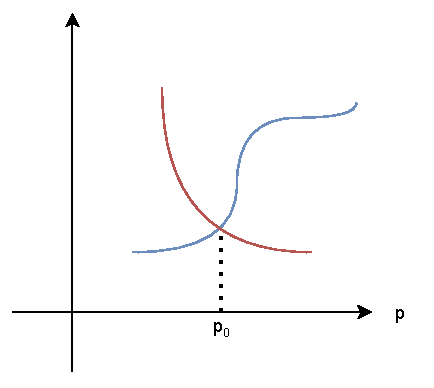
\includegraphics[scale = 0.6]{img/grap2.pdf}
    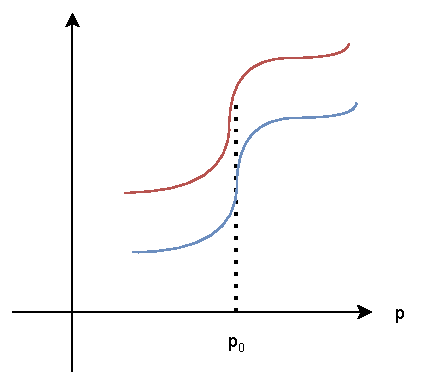
\includegraphics[scale = 0.6]{img/grap3.pdf}
    \caption{Grafici usati nella dimostrazione \textbf{da capire come}}
  \end{figure}
\end{proof}
L'unità di misura dell'informazione varia a seconda della base del logaritmo.\\
Si ha che $\log_2$ è l'unità di misura se ho a che fare con i bit (anche se
all'inizio 0 e 1 erano detti \textit{binit}) Misuro quindi in \textit{bit}. \\
Se ho $\log_e=\ln$ misuro in \textit{nat}.\\
Se ho $\log_{10}$ misuro in \textit{Hartley}.\\
La sorgente $s$ quindi emette il simbolo $s_i$ con $p_i$ e produce una quantità
di informazione pari a:
\[I(p_i)=\log_2\frac{1}{p_i}\]
e questo per ogni simbolo.\\
Si ha anche la quantità di informazione media della sorgente, facendo la media
pesata con le probabilità. Questa è detta \textbf{entropia} $H$:
\[H(S)=\sum_{i=1}^qp_i\cdot I(p_i)=\sum_{i=1}^qp_i\cdot \log_2\frac{1}{p_i}\]
spesso si usa $H_b$ con $b$ pari alla base del logaritmo, quindi:
\[H_2(S)=\sum_{i=1}^qp_i\cdot I(p_i)=\sum_{i=1}^qp_i\cdot \log_2\frac{1}{p_i}\]
Con $H_2$ funzione che ha in input tutte le probabilità:
\[H(p_1,\ldots,p_q)\]
che per praticità indichiamo con, per $S$ sorgente:
\[H(S)\]
Un altro modo di indicarla è (spesso per motivi tipografici):
\[H_2(S)=-\sum_{i=1}^qp_i\cdot \log_2{p_i}\]
Sempre dietro $H$ si ha uno scopo tipografico, non si usa $E$ in quanto sarebbe
ambiguo con \textit{energia}. Si è pensato ad usare la $\eta$ ma era comunque
scomodo da usare in documenti dattiloscritti, prima che Knuth arrivasse con \TeX
e \LaTeX.\\
La storia dietro il nome ``entropia'' era stato anche trattato con Von Neumann,
in quanto Shannon temeva fosse un termine errato, vedendo che fosse simile
all'entropia della termodinamica ma non essendo sicuro della cosa.\\
Vediamo un \textit{esperimento mentale}, detto \textbf{esperimento del
  diavoletto di Maxwell}, per dimostrare come l'entropia di Shannon e quella
della termodinamica siano effettivamente collegate tra loro. Si immagina di
avere un contenitore da cui non può uscire nulla e nemmeno in cui può entrare
nulla. Tale contenitore contiene un gas con una certa quantità di calore. Tale
contenitore è diviso in due con a metà uno sportello che si apre e chiude. Il
gas è formato da molecole che si muovono e si scontrano tra loro e contro le
pareti. Il calore è legato alla velocità di queste molecole. Lo sportello è
azionato da un ''diavoletto'' che riesce a vedere le particelle e di misurarne
la velocità. Quando vede una particella veloce la manda da una parte del
contenitore se lenta dall'altra (aprendo e chiudendo lo sportello), dividendo
così particelle lente e veloci nelle due sezioni del contenitore. Dopo un po' di
tempo tutte le particelle veloci sono da una parte e le lente dall'altra, avendo
una metà più calda (dove sono quelle veloci) e uno più freddo. Il diavoletto ha
quindi lavorato per andare contro il secondo principio della termodinamica, che
imporrebbe un miscuglio uniforme tra particelle lenti e veloci. Ma questo
principio sarebbe inviolabile quindi siamo di fronte ad un paradosso. La
soluzione al paradosso è il rapporto tra le due entropie, quella di Shannon
della teoria dell'informazione e quella della termodinamica. Il diavoletto
ha lavorato contro il secondo principio della termodinamica ma per capire se una
particella è veloce ne ha fatto una misurazione e ne ha ricavato un'informazione
sulla misura. Tale misurazione è il risultato di un evento statistico, a seconda
della particella ho velocità alta/bassa etc$\ldots$ con una certa probabilità. A
tali probabilità si associa l'entropia di Shannon e facendo i conti si scopre
che comunque il sistema è chiuso e che il diavoletto non sta facendo un lavoro
impossibile (i dettagli del discorso non vengono trattati).\\
Quindi la sorgente, ad ogni colpo di clock, emette un simbolo con una certa
quantità di informazione. \\
Un altro modo per vedere che l'entropia è una sorta di media è prendere la
sorgente $S$ e considerare messaggi di lunghezza $n$. Voglio avere $n\cdot p_i$
volte $s_i$, avendo: 
\[P=p_1^{n\cdot p_1}\cdot p_1^{n\cdot p_2}\cdot \ldots \cdot p_q^{n\cdot
    p_q}=(p_1^{p_1}\cdots p_q^{p_q})^n\]
ma allora:
\[\log_\frac{1}{P}=log_2\left[\frac{1}{p_1^{p_1}\cdots
      p_q^{p_q}}\right]=n\sum_{i=1}^q\log_2\left(\frac{1}{p_i}\right)^{p_1}=n\cdot
  \sum_{i=1}^qp_i\log_2\frac{1}{p_1}=n\cdot H_2(S)\]
\subsection{Robustezza codici di Huffman}
Sia data una sorgente $S$ con simboli $s_i$ e probabilità $p_i$ (potrei anche
non sapere che simboli emette la sorgente $S$, come se fosse una \textit{black
  box}). Le probabilità in realtà non si conoscono. Si supponga di 
poter osservare solo i simboli emessi dalla sorgente senza sapere nulla di come
è fatta. Non conosco quindi le probabilità vere ma posso solo stimarle. Chiamo
$p_i'$ tali stime. Ci si chiede quanto cambia la lunghezza media del codice
istantaneo applicando Huffman con le $p_i'$. Si ha quindi:
\[L'=\sum_{i=1}^q p_i'l_i\]
anziché:
\[L=\sum_{i=1}^q p_il_i\]
Cercando di capire quanto si discostano $L$ e $L'$.\\
Presi gli errori $e_i$ commessi per stimare $p_i'$ ho che:
\[p_i'=p_i+e_i\]
Si segnala che $e_i$ può essere positivo, negativo o nullo.\\
Sia $p_1,\ldots, p_q$ che $p_1',\ldots, p_q'$ sono distribuzioni di probabilità
e quindi $\sum_{i=1}^q p_i=1$.\\
Quindi:
\[\sum_ip_i'=\sum_i (p_i+e_i)=\sum_{i=1}^q p_i+\sum_{i=1}^q +e_i=1+\sum_{i=1}^q
  +e_i=1\] 
dato che $\sum_ip_i'=1$. Ne segue quindi per forza vale che:
\[\sum_i e_i=0\]
e quindi la media degli errori è:
\[\frac{1}{q}\sum_{i=1}^q e_i=0\]
e che la varianza degli errori vale
\[\sigma^2=\frac{1}{q}\sum_{i=1}^q e_i^2\]
Per la lunghezza media ho che:
\[L'=\sum_{i=1}^q p_i'\cdot l_i=\sum_{i=1}^q p_i\cdot l_i=\sum_{i=1}^q e_i\cdot
  l_i=L+\sum_{i=1}^q e_i\cdot l_i\]
Quindi la variazione tra le lunghezze medie ottenute con Huffman usando $p_i'$ e
$P_i$ è:
\[\sum_{i=1}^q e_i\cdot l_i\]
Voglio quindi minimizzare $\sum_{i=1}^q e_i\cdot l_i$. Cerchiamo quindi gli
$e_1,\ldots e_q$ tali per cui la funzione:
\[f(e_1,\ldots e_q)=\sum_{i=1}^q e_i\cdot l_i\]
è minima.\\
Cerco quindi i punti stazionari tramite le derivate parziali rispetto alle
variabili $e_i$ per poi porle a 0. Vogliamo che la media dei valori assunti da
$e_i$ si nulla e che la varianza $\sigma^2$ assuma un valore fissato imponendo i
seguenti vincoli:
\[\frac{1}{q}\sum_{i=1}^q e_i=0\implies \sum_{i=1}^q e_i=0\]
e:
\[\frac{1}{q}\sum_{i=1}^q e_i^2-\sigma^2 =0\]
Per risolvere questo problema di ottimizzazione vincolata utilizziamo i
\textbf{moltiplicatori di Lagrange}. Abbiamo due vincoli e quindi usiamo due
moltiplicatori: $\mu$ e $\lambda$:
La funzione u cui calcolare i punti stazionari diventa:
\[\mathcal{L}(e_1,\ldots,e_q)=\sum_{i=1}^qe_il_i-\lambda\sum_{i=1}^q
  e_i-\mu\left(\sum_{i=1}^q e_i^2-\sigma^2\right)\] 
Calcolo quindi le derivate parziali rispetto a $e_i$ e le pongo nulle:
\[\frac{\partial\mathcal{L}}{\partial e_i}=l_i-\lambda-\frac{2\mu}{q}e_i=0\]
e sommando queste equazioni ho:
\[\sum_{i=1}^q l_i-\lambda q-\frac{2\mu}{q}\sum_{i=1}^q e_i=0\]
e avendo che $\sum_{i=1}^qe_i=0$ ottengo:
\[\sum_{i=1}^q l_i-\lambda q=0\]
e quindi:
\[\lambda=\frac{1}{q}\sum_{i=1}^q l_i\]
Cerchiamo quindi il valore di $\mu$.
Ricordando che:
\[\frac{\partial\mathcal{L}}{\partial e_i}=l_i-\lambda-\frac{2\mu}{q}e_i=0\]
sommo le equazioni moltiplicando la prima per $e_1$, la seconda per $e_2 $
etc$\ldots$:
\[\sum_{i=1}^q e_il_i-\lambda \sum_{i=1}^q e_i-\frac{2\mu}{q}\sum_{i=1}^q e_i^2=0\]
e avendo che $\sum_{i=1}^qe_i=0$ ottengo:
\[\sum_{i=1}^q e_il_i-2\mu\sigma^2=0\]
da cui:
\[\mu=\frac{1}{2\sigma^2}\sum_{i=1}^qe_il_i\]
Ricordando che:
\[\frac{\partial\mathcal{L}}{\partial e_i}=l_i-\lambda-\frac{2\mu}{q}e_i=0\]
sommo le equazioni moltiplicando la prima per $l_1$, la seconda per $l_2 $
etc$\ldots$:
\[\sum_{i=1}^q l_i^2-\lambda \sum_{i=1}^q l_i-\frac{2\mu}{q}\sum_{i=1}^q
  e_il_i=0\]
Sostituisco $\lambda$ e $\mu$:
\[\sum_{i=1}^q l_i^2- \frac{1}{q}\left(\sum_{i=1}^q l_i\right)^2-
  \frac{1}{2q\sigma^2}\left(\sum_{i=1}^qe_il_i\right)^2=0\]
Ma allora:
\[\left(\sum_{i=1}^qe_il_i\right)^2=\sigma^2\left[q\sum_{i=1}^q
    l_i^2-\left(\sum_{i=1}^q
      l_i\right)^2\right]=\]
\[\sigma^2q^2\left[\frac{1}{q}\sum_{i=1}^q
    l_i^2-\left(\frac{1}{q}\sum_{i=1}^q l_i\right)^2\right]=\sigma^2q^2\cdot v\]
con $v$ varianza delle $l_i$.\\
Dato che $q^2$ e $\sigma^2$ sono fissate bbiamo trovato che il quadrato della
variazione tra le lunghezze medie, ovvero il quadrato di $f(e_1,\ldots,e_q)$ che
volevamo minimizzare, è direttamente proporzionale alle lunghezze delle
codeword. Quindi si minimizza mettendo in alto il nuovo simbolo in quanto si
minimizza la varianza rendendo più \textbf{robusto} il codice, ovvero meno
sensibile ad errori sulle probabilità (perlomeno ragionando in ottica di
lunghezza media).\\
Quando esce il simbolo $s_i$ abbiamo quindi $I(p_i)=\log_r \frac{1}{p_i}$, con
tipicamente $r=2$, misurando la quantità di informazione in bit.\\
Studiamo ora proprietà di $H_2(S)$, che può essere studiata come una
funzione. Si nota in primis che $p=0$ è escluso (avendo una discontinuità del
terzo tipo) e $p=1$ incluso. Avendo:
\[H_2(S)=\sum_{i=1}^q p_i\log_2\frac{1}{p_i}=H_2(p_1,\ldots, p_q)\]
che graficamente è:
\begin{figure}[H]
  \centering
  \begin{tikzpicture}
    \begin{axis}[axis lines = left, xlabel=$p$, ylabel=$p\log_2\frac{1}{p}$,
      xmin=0,xmax=1, ymax=0.7, samples=300] 
      \addplot[black, ultra thick, domain=0:1,] {x*log2(1/x)};
    \end{axis}
  \end{tikzpicture}
\end{figure}
Ma questo è scomodo quindi riscrivo $\frac{1}{p}$ in modo che anche l'origine
sia inclusa. \\
Sappiamo quindi che:
\[H_S(S)\geq 0\]
e vale 0 sse $H_2(p_1,\ldots, p_q)=0$ e quindi una certa $p_i=0$ e quindi tutte
le altre $p_j$ sono anch'esse nulle.
Cerchiamo ora il massimo.\\
Usiamo la \textbf{disuguaglianza di Gibbs}.
\begin{teorema}[Disuguaglianza di Gibbs]
  Disegnano il logaritmo naturale (anche se vale per ogni base) e
  una retta $r$ che è tangente alla funzione in $1$:
  \begin{figure}[H]
    \centering
    \begin{tikzpicture}
      \begin{axis}[axis lines = left, samples=300, ymin=-4] 
        \addplot[black, ultra thick,] {ln(x)};
        \addplot[blue, ultra thick,] {x-1};
      \end{axis}
    \end{tikzpicture}
  \end{figure}
  Si scopre quindi che:
  \[\ln (x)\leq x-1\]
  e vale l'uguaglianza sse $x=1$.\\
  Prendo quindi due distribuzioni $x_1,\ldots, x_q$ e $y_1,\ldots, y_q$. La
  disuguaglianza afferma che:
  \[\sum_{i=1}^q x_i\log_2\left(\frac{y_i}{x_i}\right)\leq 0\]
\end{teorema}
\begin{proof}
  Dimostriamo questa disuguaglianza. Ho che, tramite cambio base:
  \[\sum_{i=1}^q
    x_i\log_2\left(\frac{y_i}{x_i}\right)=\frac{1}{\log_2}\sum_{i=1}^q
    x_i\ln\left(\frac{y_i}{x_i}\right)\leq \frac{1}{\log_2}\sum_{i=1}^q
    x_i\left(\frac{y_i}{x_i}-1\right)=\frac{1}{\ln 2}\sum_{i=1}^q y_i-x_i\]
  \[=\frac{1}{\ln 2}\left(\sum_{i=1}^q y_i-\sum_{i=1}^q x_i\right)=\frac{1}{\ln
      2}(1-1)=0\]
  e quindi vale la disuguaglianza di Gibbs.\\
  L'unica volta che abbiamo maggiorato abbiamo usato $\ln x\leq x-1$ che ci
  dice che vale $0$ sse  $x=1$ e quindi vale l'uguaglianza sse
  $\frac{y_i}{x_i}=1$, quindi se le due distribuzioni coincidono, con
  $x_i=y_i,\forall i$.
\end{proof}
Cerco quindi il massimo dell'entropia. Dimostro che:
\[\max H_2(p_1,\ldots, p_q)=\log_2 p\]
Per farlo uso Gibbs:
\[H_2(S)-\log_2 q=\left(\sum_{i=1}^q p_i\log_2\frac{1}{p_i}\right)-log_2 q\]
ma voglio includere tutto nella sommatoria, lo moltiplico per una sommatoria che
fa 1:
\[=\left(\sum_{i=1}^q p_i\log_2\frac{1}{p_i}\right)-log_2 sum_{i=1}^qp_i\]
ora lo posso includere
\[=\sum_{i=1}^q p_i\log_2\frac{1}{p_i}- sum_{i=1}^qp_i log_2\]
e quindi:
\[\sum_{i=1}^qlog_2\frac{1}{p_i}-log_2 q\]
e quindi:
\[=\sum_{i=1}^q p_i\log_2\frac{1}{p_i\cdot q}=\sum_{i=1}^q
  p_i\log_2\frac{\frac{1}{q}}{p_i}\]
Dove posso riconoscere Gibbs, con $\frac{1}{q}$ che è una distribuzione
uniforme e $p_i$ è l'altra distribuzione. Quindi:
\[H_2(S)-\log_2 q=\frac{1}{\ln 2}\sum_{i=1}^q\leq 0\]
possiamo dire che:
\[H_2(S)\leq \log_2 q\]
Inoltre vale 0 sse $p_i=\frac{1}{q},\forall i$, quindi se ho una distribuzione è
uniforme, con quindi $\log_2 q$ come massimo.\\
Un'applicazione di questo calcolo è la relazione tra entropia e lunghezza media
di un codice e quindi con la codifica di sorgente.\\
Si prende una sorgente con $q$ simboli $s_i$, con probabilità $p_i$. Si supponga
di avere codeword $l_i$ per un codice istantaneo. Ho la disuguaglianza di Kraft,
con $K\leq 1$:
\[K=\sum_{i=1}\frac{r^{l_i}}\leq 1\]
Definisco, $\forall i\in\{1,\ldots, q\}$:
\[Q_i=\frac{r^{-l_i}}{K}\]
I vari $Q_i$ sono $\in[0,1]$ e quindi le posso considerare singolarmente come
probabilità. Vedo che:
\[\sum_{i=1}^q Q_i=\sum_i \frac{r^{-l_i}}{K} = \frac{1}{K}\sum_i
  r^{-l_i}=\frac{1}{K}K =1\]
e quindi sono una distribuzione di probabilità.\\
Uso quindi Gibbs:
\[\sum_{i=1}^q p_i\log_2\frac{Q_i}{p_i}\leq 0\]
Ho che, spezzando il logaritmo:
\[\sum_{i=1}^q p_i\log_2\frac{Q_i}{p_i}=\sum_{i=1}^qp_i\left(
  \log_2\frac{1}{p_i}-\log_2\frac{1}{Q_i}\right)\]
\[=H_2(S)-\sum_{i=1}^qp_i\log_2\frac{1}{Q_i}\leq 0\]
Ma quindi:
\[H_2(S)\leq  \sum_{i=1}^qp_i\log_2\frac{1}{Q_i}=\sum_{i=1}^qp_i\log_2
  \frac{K}{r^{-l_i}}=\sum_{i=1}^qp_i\left(\log_2K - \log_2 r^{-l_i}\right)\]
\[=\log_2 K\sum_{i=1}^qp_i+\sum_{i=1}^qp_i l_i\log_2 r\]
\[
  =\log_2 K+\log_2 r\sum_{i=1}^qp_i l_i\log_2 r=\log_2 K+L(log_2 r)\leq L\log_2
  r\]
in quanto $\log_2 K\leq 0$ (essendo $K\leq 1$ per Kraft).\\
Quindi:
\[H(S)\leq L\log_2 r\]
E $\log_2 r$ è una costante che fa cambiare la base del logaritmo:
\[\frac{H_2(S)}{log_2 r}\leq L\]
ma quindi:
\[H_r(S)\leq L\]
Quindi partendo da una sorgente in cui si ipotizza un codice istantaneo possiamo
dire che la lunghezza media deve essere maggiore uguale dell'entropia della
sorgente su base r-aria, dove $r$ è il numero di simboli dell'alfabeto di
codifica. Il fatto che la lunghezza media non può essere minore dell'entropia
(quindi della quantità media di informazione)
si può interpretare dicendo che la quantità media di informazione associata al
messaggio è quella che non posso rappresentare in modo più compatto, mi da un
limite. La sorgente quindi, ogni volta che emette un simbolo, emette mediamente
una certa quantità di9 informazione e quindi ogni messaggio ha una quantità di
informazione che è la somma di quelle di ciascun simbolo. La quantità di
informazione del messaggio è quella che non posso rappresentare in maniera più
compatta con un codice istantaneo. Ho una sorta di limite e se codificassi con
una lunghezza media più bassa perderei informazione. Posso vedere il codice
istantaneo come una compressione dei dati senza perdita di informazione, a meno
di ulteriori compressioni.\\
\textit{Se avessi sorgenti con memoria avrei che si avrebbero vincoli che
  abbassano l'entropia.} \\
Immagino ora una sorgente con due simboli $s_1$ e $s_2$, con $p_1+p_2=1$ e
quindi $p_1=1-p_2$ e quindi mi basta la probabilità di uno solo dei due simboli
che chiamo $p$. Posso dire che:
\[H_2(S)=p\log_2\frac{1}{p}+(1-p)\log_2\frac{1}{1-p}\]
Questa tipologia di sorgente è una \textbf{sorgente Bernoulliana} che è del
tipo, con la derivata che si annulla in $\frac{p}{2}$:
\begin{figure}[H]
  \centering
  \begin{tikzpicture}
    \begin{axis}[axis lines = left, xlabel=$p$,
      ylabel=$p\log_2\frac{1}{p}+(1-p)\log_2\frac{1}{1-p}$,,xmin=-0.1,xmax=1.1,
      ymax=1.1, samples=600] 
      \addplot[black, ultra thick, domain=0:1,]
      {x*log2(1/x)+(1-x)*log2(1/(1-x))};
      \addplot[thick,dashed,blue,]
      coordinates {(0.5,0)(0.5,1)};
    \end{axis}
  \end{tikzpicture}
\end{figure}
in questo caso $p=1$ sarebbe escluso ma lo completo dicendo che vale 0 in $p=1$
tramite una sostituzione. Stesso discorso per $p=0$. \\
Il valore massimo è appunto $p=\frac{1}{2}$ e quindi si ha che:
\[H_2\left(\frac{1}{2}\right)=1\]
Si vuole rappresentare la sequenza di simboli in modo efficiente, ovvero con
lunghezza media minima. Vogliamo quindi la rappresentazione più compatta
possibile, pensando al codice istantaneo dal punto di vista della compressione
senza perdita di informazione, avendo che il ricevente può risalire alla
sequenza di simboli inviata e compressa.\\
Parlando di codifica di sorgente si ha un simbolo per ogni colpo di
clock. Possiamo pensare ad un codice istantaneo per comprimere le sequenze di
simboli emesse dalla sorgente, compressione senza perdita di informazione,
\textbf{compressione lossless} con il
ricevente che riceve e capisce perfettamente la sequenza di partenza. La
compressione dipende dalla ridondanza.
\textit{Si hanno altri tipi di compressione, \textbf{lossy}, vedisi MP3 o MPEG,
  dove la compressione ha perdita di informazione.}\\
Un metodo di compressione ottimale comprime fino a raggiungere l'entropia della
sorgente, non lasciando nulla di ``inutile'', garantendo però la
ricostruzione. Con compressione si ha un codice istantaneo e dobbiamo dire al
destinatario quale sia l'albero di decodifica. \\
Grazie a McMillan sappiamo che la disuguaglianza di Kraft vale anche per i
codici univocamente decodificabili. Tutto quanto detto tramite Gibbs riottengo
ancora:
\[H_r(S)\leq L\]
che quindi vale per tutti i codici univocamente decodificabili.\\
\section{Codifica di Shannon-Fano}
Shannon e Fano si chiedono se la quantità di informazione r-aria, con quindi
alfabeto r-ario, è minore uguale
della lunghezza del simbolo, avendo sempre simboli $s_i$, con $p_i$ e $l_i$:
\[\log_r\frac{1}{p_i}\leq l_i\]
Vogliamo che $l_i$ sia il più piccolo ovvero l'unico compreso in:
\[\log_r \frac{1}{p_i}\leq l_i< \log_r\frac{1}{p_i}+1\]
Questo intervallo ha ampiezza 1 e contiene un solo intero.\\
Calcolo gli $l_i$ in modo che rispettino questo principio. Tali lunghezze sono
le \textbf{lunghezze di Shannon-Fano}.\\
Ragioniamo sulle lunghezze e vediamo se si ha un codice istantaneo con quelle
lunghezze. 
Facendo:
\[r^{\log_r \frac{1}{p_i}}\leq r^{ l_i}< r^{\log_r\frac{1}{p_i}+1}\]
ma allora:
\[ \frac{1}{p_i}\leq r^{l_i}< r^{\log_r\frac{1}{p_i}}r\]
che è:
\[ \frac{1}{p_i}\leq r^{l_i}< \frac{1}{p_i}r\]
Faccio il reciproco:
\[p_i\geq \frac{1}{r^{l-i}}> \frac{p_i}{r}\]
Ora sommo tutti questi $l_i$:
\[\sum_{i=1}^qp_i\geq \sum_{i=1}^q\frac{1}{r^{l-i}}>\sum_{i=1}^q \frac{p_i}{r}\]
ma quindi è:
\[1\geq K> \frac{1}{r}\]
Anche se in realtà mi basta la prima parte:
\[1\geq K\]
\textbf{Si ha quindi un codice istantaneo con le lunghezze di
  Shannon-Fano}. Potrei dire lo stesso per un codice univocamente decodificabile
ma conviene ovviamente un codice istantaneo.\\
Passo ad ``ottimizzare'' le singole lunghezze e non la media delle stesse.\\
Ci si chiede ora se si ottiene una lunghezza media ottimale, ``sfidando''
Huffman, che solo all'ultimo ottiene le codeword che ottimizzano la lunghezza
media, facendo un ragionamento che comprende tutte le probabilità facendo la
scelta migliore per l'intera sorgente.  \\
Con la codifica di Shannon-Fano si ha che ogni lunghezza dipende dalla singola
probabilità e sfrutta un algoritmo più performante di quello di Huffman ma si
ottiene un \textbf{codice non ottimale} e vedremo di quanto ci si discosta. Per
ottenere le codeword poi parto dalle lunghezze di Shannon-Fano e ragiono sugli
alberi di decodifica, costruendone uno per scegliere le codeword. Ci si può
anche chiedere quali sono le lunghezze che consentono di dare un nome univoco a
ciascun evento che si possa verificare, astraendo dalle sorgenti e arrivando al
nocciolo dell'essenza dell'informazione. \\
Ripartiamo dalle lunghezze di Shannon-Fano:
\[\log_r \frac{1}{p_i}\leq l_i< \log_r\frac{1}{p_i}+1\]
Voglio ottenere dei limiti per la lunghezza media, ricordando che:
\[L=\sum_{i=1}^q p_il_i\]
ricostruisco quindi la disequazione delle lunghezze per ottenere i limiti della
lunghezza media.\\
Moltiplico per $p_i$:
\[p_i\log_r \frac{1}{p_i}\leq p_il_i<p_i \log_r\frac{1}{p_i}+p_i\]
e sommo tutto:
\[\sum_{i=1}^qp_i\log_r \frac{1}{p_i}\leq \sum_{i=1}^qp_il_i<\sum_{i=1}^qp_i
  \log_r\frac{1}{p_i}+\sum_{i=1}^q p_i\] 
Ma è:
\[H_r(S)\leq L< H_r(S)+1\]
Avendo ottenuto i limiti superiore e inferiore (anche se quello inferiore già si
sapeva, visto che $H_r(S)\leq L$ valeva per tutti i codici univocamente
decodificabili e per quelli istantanei). I codici di Huffman hanno lunghezza
media minore, essendo ottimali, di quelli di Shannon-Fano. Vedo quindi che
Shannon-Fano dista di 1 dall'ottimo ma non sempre è così buono. Vediamo un
esempio con due simboli:
\[p_1=1-\frac{1}{2^j}\mbox{ e }p_2=\frac{1}{2^j}\]
per $j\geq 2$ fissato.\\
Si ha che il secondo simbolo esce raramente.\\
Calcolo le lunghezze di Shannon-Fano:
\[\log_2\frac{1}{p_2}\leq l_2\to \log_2 2^j\leq l_2\to l_2=j\]
\[\log_2\frac{1}{p_1}\leq l_2\to\log_2\frac{2^j}{2^j-1}\leq\log_2\left( 1+ l_2\to
    \frac{1}{2^j-1}\right)\leq l_2\to 1\leq l_1\to l_1=1\]
Si noti che Huffman darebbe lunghezza 1 ad entrambe mentre Shannon-Fano 1 e $j$
e quindi sono ben lontane da essere ottime, anche se la lunghezza media dista al
più 1 da quella ottima (questo per l'intervento nel conto delle probabilità di
uscita dei simboli). Posso comunque poi accorciare gli alberi con nodi interni
inutili, soprattutto con alfabeto binario. Quindi pur non essendo ottimo è
comunque accettabile.\\ 
Possiamo dire che si ha una tendenza verso l'ottimo con la codifica di
Shannon-Fano.
\begin{definizione}
  %mettere figura
  Definisco l'n-sima estensione $S^n$ di una sorgente $S$, con $n\geq 1, n\in
  \mathbb{N}$, Per $n=1$ l'estensione coincide con $n$. Per $n>1$ immagino di
  avere $n$ copie della sorgente che lavorano in parallelo in modo sincrono,
  quindi con un colpo di clock unico per tutte. La prima sorgente emette
  $s_{i1}$, la seconda $s_i2$ e l'ultima $s_{in}$. L'n-esima estensione
  considera questi $s_{ij}$ come un vettore, considerando le $n$ copie come una
  singola sorgente $S^n$ che ha come alfabeto i simboli $\sigma_1,
  \ldots,\sigma_m$, con $\sigma_i=\{s_{i1},\ldots, s_{in}\}$, dove ogni $s_i$ è
  lungo $j$ e quindi $m=q^n$. \\
  Ho che:
  \[Prob[\sigma_i]=p_{i1}\cdot p_{i2}\cdot \ldots p_{in}\]
  Questa probabilità e $q^n$ sono due problematiche, più è grande l'estensione e
  più simboli si dovrà costruire (con limiti anche macchina). Se ho probabilità
  piccole come $p_{ij}$ moltiplicandoli diventano ancora più piccoli.\\
  Si ha quindi un codice istantaneo con $q^n$ simboli che sono n-uple di simboli
  della sorgente di partenza, che in ogni $\sigma_i$ possono essere
  mescolati. \\
  Ogni singolo $S$ ha un $H_r(S)$ quindi si ha che, valendo l'additività per
  l'entropia: 
  \[H_r(S^n)=n\cdot H_r(S)\]
  
\end{definizione}
\begin{teorema}[Primo teorema di Shannon, noiseless coding theorem]
  Avendo:
  \[H_r(S)\leq L< H_r(S)+1\]
  Si ha che vale qualunque sia la sorgente e qualunque sia il codice
  istantaneo.\\
  In particolare, per $n\geq 1$ vale anche per l'n-esima estensione:
  \[H_r(S^n)\leq L_n< H_r(S^n)+1\]
  Con $L_n$ lunghezza media del codice per $S^n$. Si ha quindi che:
  \[n\cdot H_r(S)\leq L_n< n\cdot H_r(S)+1\]
  Divido per $n$, ottenendo la formula del \textbf{primo teorema di Shannon}:
  \[H_r(S)\leq \frac{L_n}{n}< H_r(S)+\frac{1}{n}\]
  Si era partiti quindi da un intervallo di ampiezza 1 per arrivare ad uno di
  ampiezza $\frac{1}{n}$, avendo lo stesso estremo di partenza mentre l'estremo
  di fine muta, in modo tale che l'ampiezza dell'intervallo decresce
  all'aumentare di $n$.
  Al crescere di $n$ quindi tale quantità viene schiacciata verso l'ottimo (a
  mo' dei 
  \textit{due carabinieri}).\\
  D'altro canto $\frac{L_n}{n}$ è la lunghezza media di un codice istantaneo che
  codifica la sorgente $S_n$, che ha come simboli elle n-uple. La codeword
  codifica tutta l'n-upla e tutte le codeword hanno lunghezza media $L_n$ e
  quindi in media servono $L_n$ bit, nel caso binario, per rappresentare la
  n-upla. Ogni singola componente della n-upla ha quindi lunghezza
  $\frac{L_n}{n}$. 
  So che, avendo $\sigma_i=\{s_{i1},\ldots, s_{in}\}$,
  ogni $s_{ij}$ ha lunghezza media $\frac{L_n}{n}$. Quindi ha senso
  confrontare 
  $H_r(S)\leq \frac{L_n}{n}< H_r(S)+\frac{1}{n}$ con $H_r(S)\leq L<
  H_r(S)+1$. Confrontando quindi, tramite la formula del primo teorema di
  Shannon, si giunge a dire che se al posto di codificare la 
  sorgente codifico le n-esime estensioni della sorgente per $n$ crescente
  allora ottengo una codifica per l'n-esima estensione che è migliore di quella
  che avevo codificando i singoli simboli della sorgente. È migliore perché ho
  un intervallo per la lunghezza media di ampiezza $\frac{1}{n}$, che quindi al
  crescere di $n$ diventa sempre più piccolo, tendendo all'ottimo.\\
  Il teorema ha validità teorica e interesse storico ma in pratica dovrei
  costruire $S^n$, con tanti 
  simboli dei quali alcuni potrebbero avere probabilità talmente bassa da essere
  difficile da rappresentare a livello macchina.
\end{teorema}
\section{Canali di Comunicazione}
Prima di parlare del \textbf{secondo teorema di Shannon} dobbiamo approfondire
il canale, in forma di modello matematico. \\
In input al canale ho simboli di un alfabeto $A$, ovvero
$a_1,a_2,\ldots,a_q$. Dal canale escono simboli di un alfabeto $B$
potenzialmente diverso, $b_1,\ldots, b_s$. Il rumore può cambiare un simbolo e
quindi il canale viene modellato con probabilità condizionate tra simbolo in
entrata e simbolo in uscita:
\[P(b_j|a_i)\]
Per queste probabilità usiamo una matrice $M$ con $q$ righe, una per ogni
simbolo di A, e $s$ colonne, una per ogni simbolo di $B$, con:
\[M_{ij}=P(b_j|a_i)\]
\end{document} 
% LocalWords:  clock burst Hamming codeword errario sottoalberi sottoalbero
% LocalWords:  Pseudocodice